%    JJJ    AA     CCCCCC KKK   K TTTTTT HH  HH EEEEEE BBBBBB UU  UU SSSSSS    CCCCCC OOOOOO MM  MM
%    JJJ   AAAA    CCCCCC KKK  K  TTTTTT HH  HH EEEEEE BB   B UU  UU SSS       CCCCCC OOOOOO MM  MM
%    JJJ  AA  AA   CC     KKK K     TT   HHHHHH EEE    BB   B UU  UU SSS       CC     OO  OO MMMMMM
%    JJJ AA    AA  CC     KKKK      TT   HHHHHH EEEEEE BBBBBB UU  UU  SSSSS    CC     OO  OO M MM M
%    JJJ AAAAAAAA  CC     KKK K     TT   HH  HH EEE    BB   B UU  UU    SSS    CC     OO  OO M MM M
% JJJJJJ AA    AA  CCCCCC KKK  K    TT   HH  HH EEEEEE BB   B UUUUUU    SSS .. CCCCCC OOOOOO M MM M
% JJJJJJ AA    AA  CCCCCC KKK   K   TT   HH  HH EEEEEE BBBBBB UUUUUU SSSSSS .. CCCCCC OOOOOO M MM M
% 
% Texte Geschrieben von Stefan Bopp und Chantal Frunz
% Mehr Informationen sind auf jackthebus.com zu finden
% 
% Beispiele für das Einfügen von Bildern
%
%\begin{wrapfigure}{R}{0.45\textwidth} 
%  \begin{centering}
%    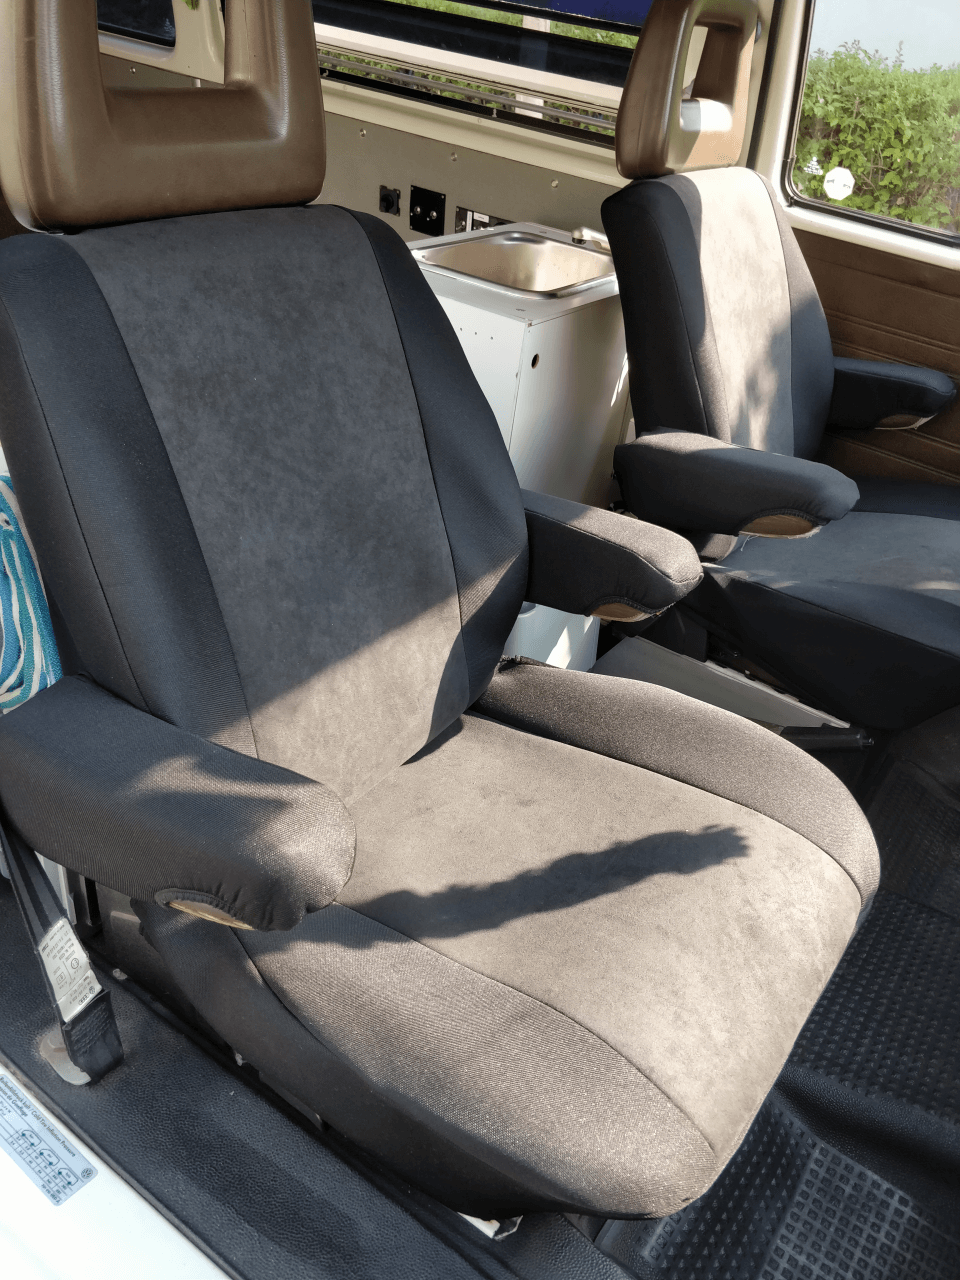
\includegraphics[width=0.4\textwidth, height=5cm, keepaspectratio]{../Bilder/Sylt/1.png}
%    \caption{Regen}
%  \end{centering}
%\end{wrapfigure} 

%\begin{figure}[b]
%   \centering
%      %\subfloat[CAPTION]{BILDERCODE}\qquad
%   \subfloat{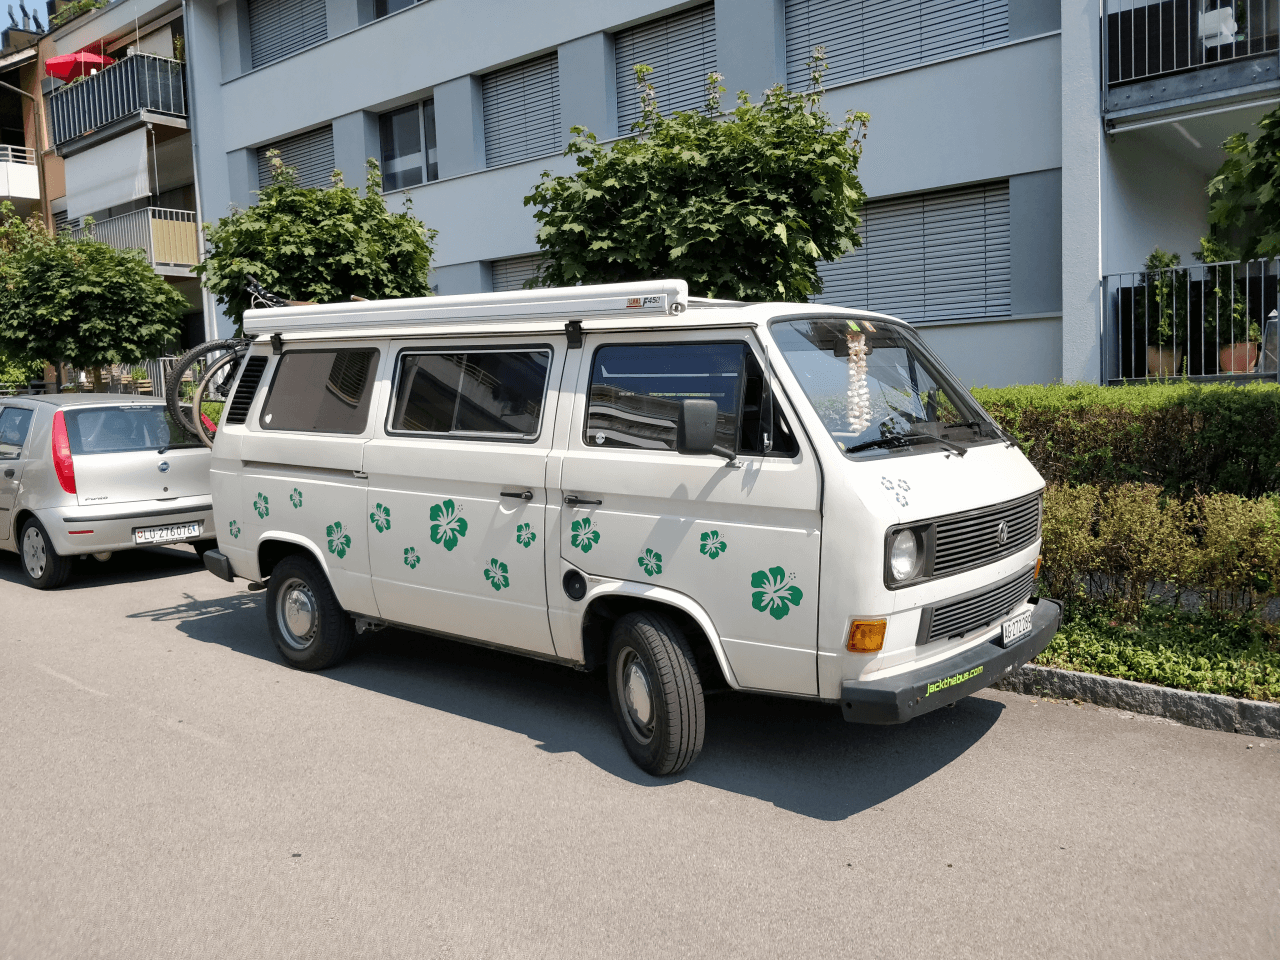
\includegraphics [width=0.3\textwidth]{../Bilder/Sylt/2.png}}\quad
%   \subfloat{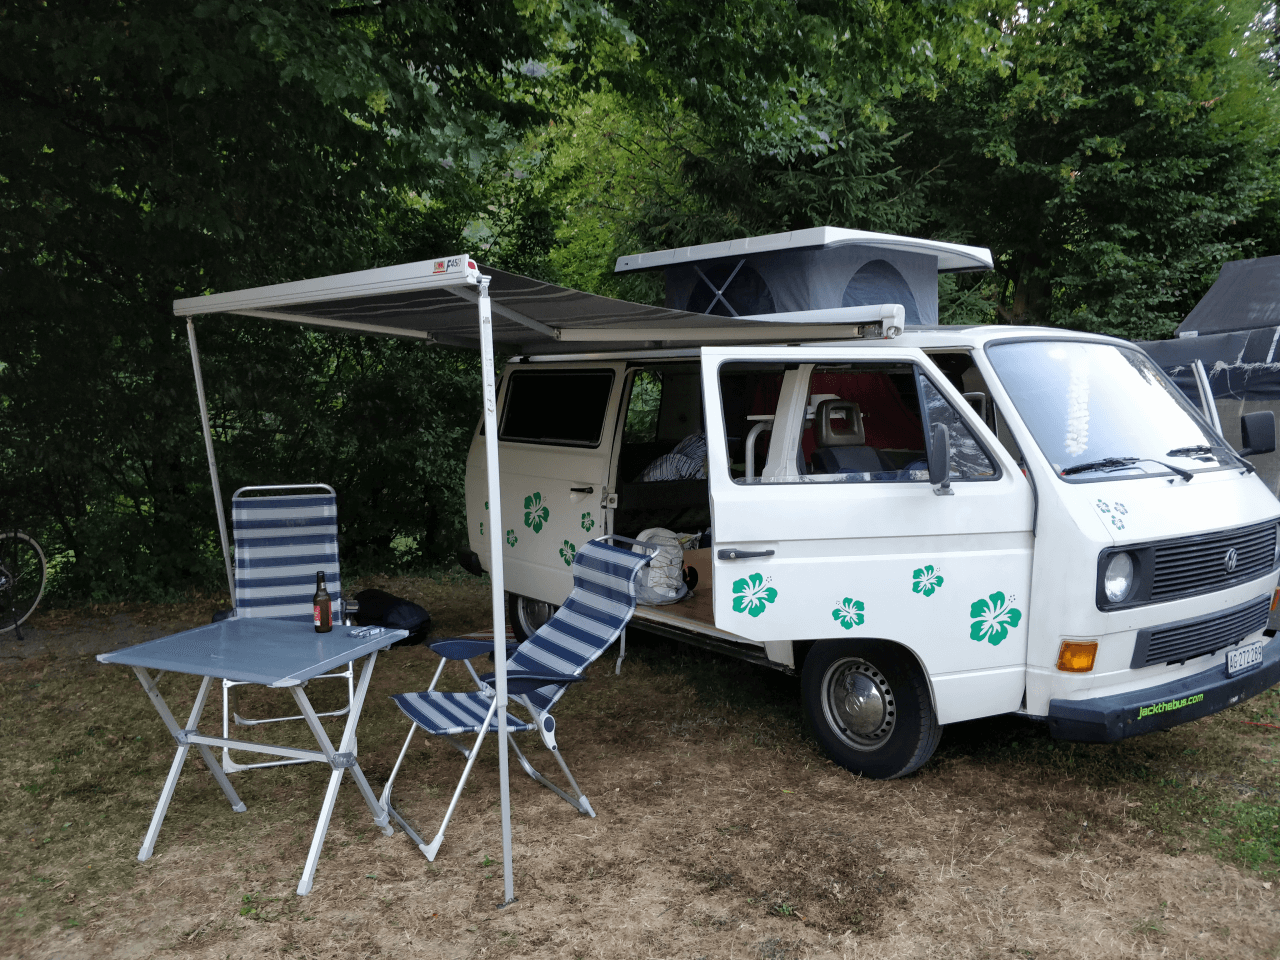
\includegraphics [width=0.3\textwidth]{../Bilder/Sylt/3.png}}\quad
%   \subfloat{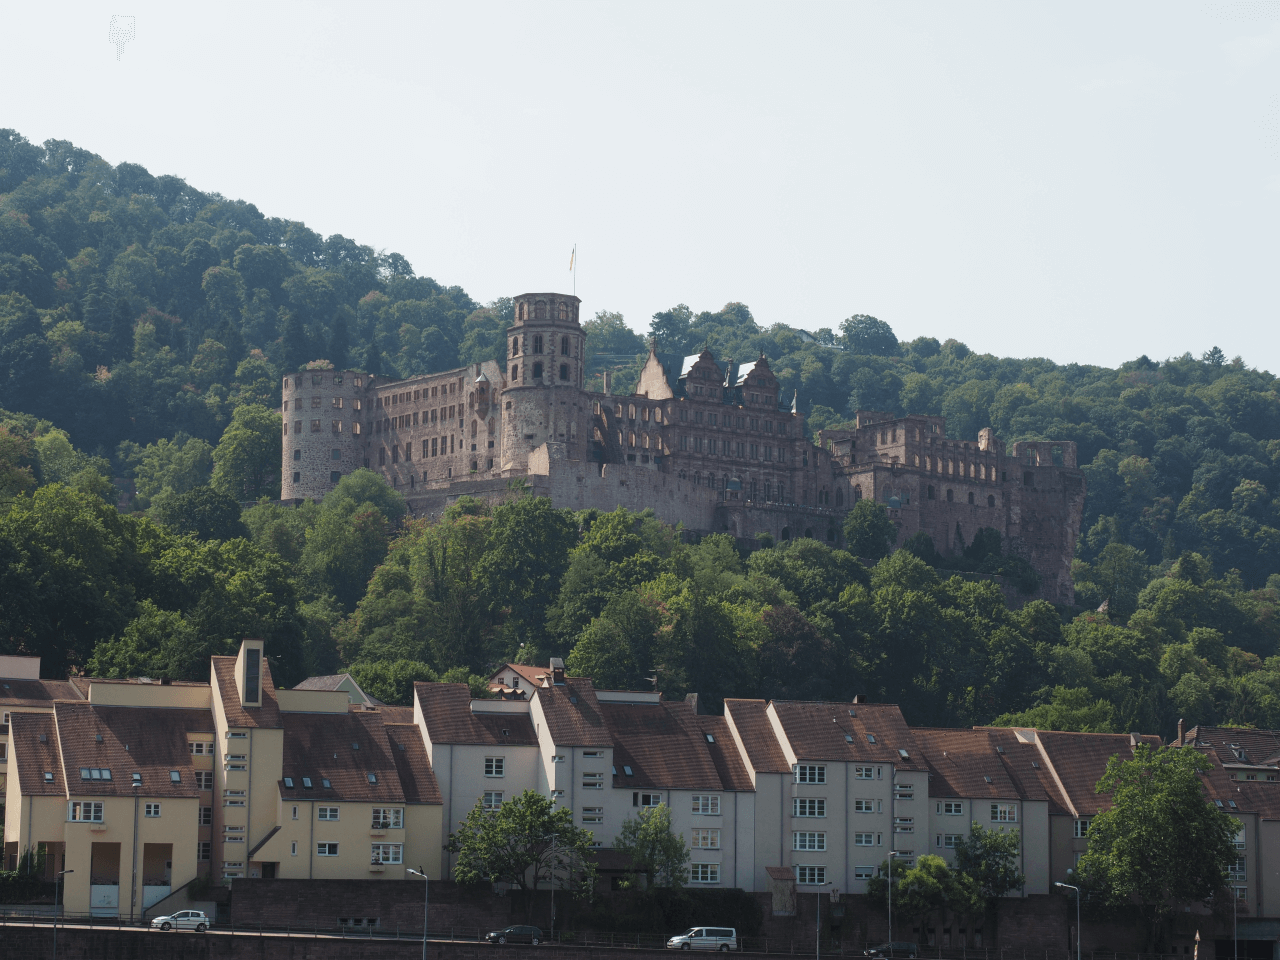
\includegraphics [width=0.3\textwidth]{../Bilder/Sylt/4.png}}\quad
%   \caption[Meran]{Meran}
%\end{figure}

%\begin{figure}[hb]
%    \centering
%    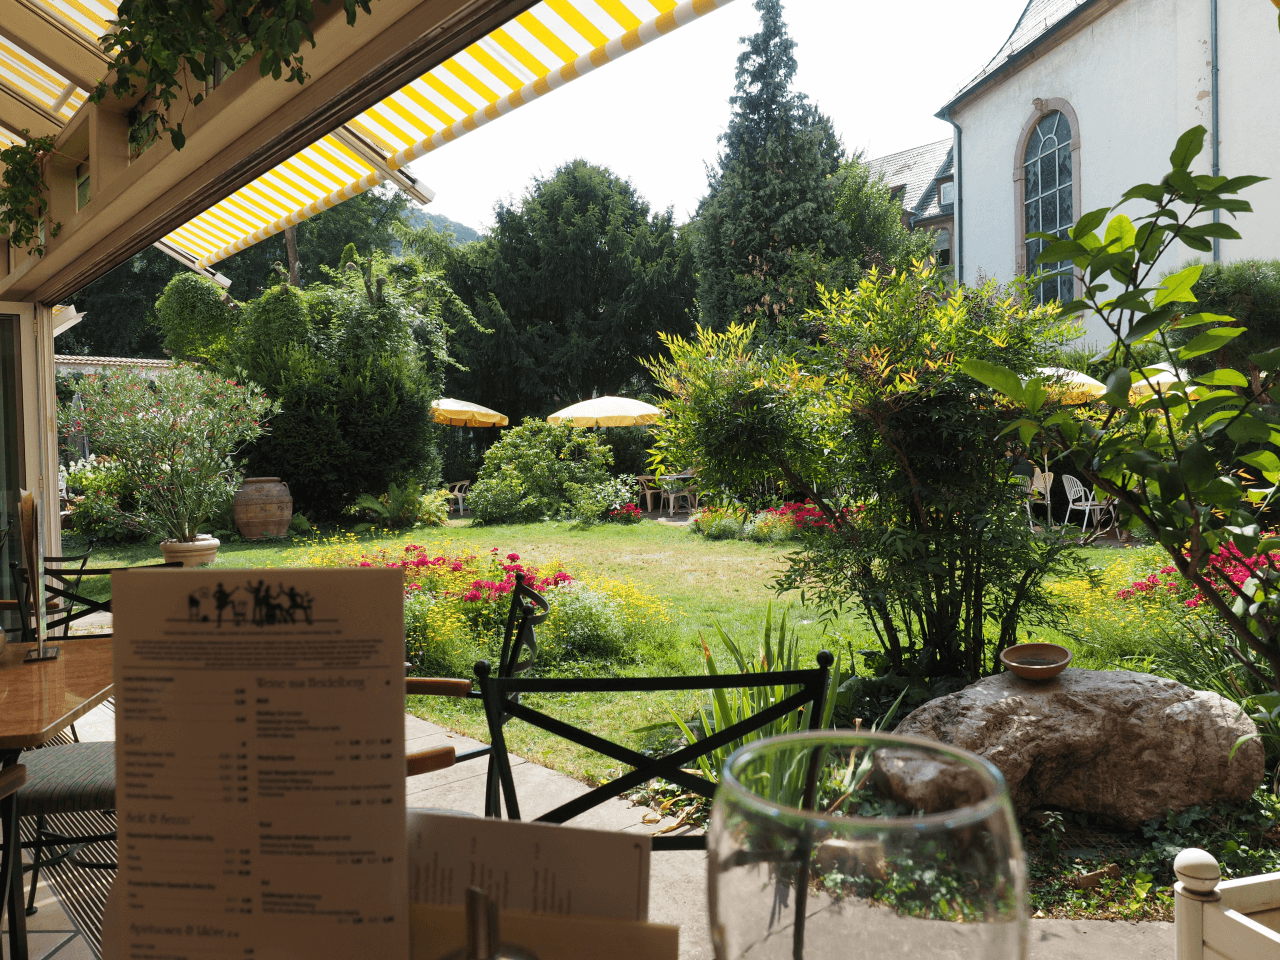
\includegraphics[width=\textwidth]{../Bilder/Sylt/7.png}
%    \caption{Da sind sie ja...}
%    \label{img:Sardinien}
%\end{figure}

\subsection{Einleitung} 

\begin{wrapfigure}{R}{0.35\textwidth} 
  \begin{centering}
    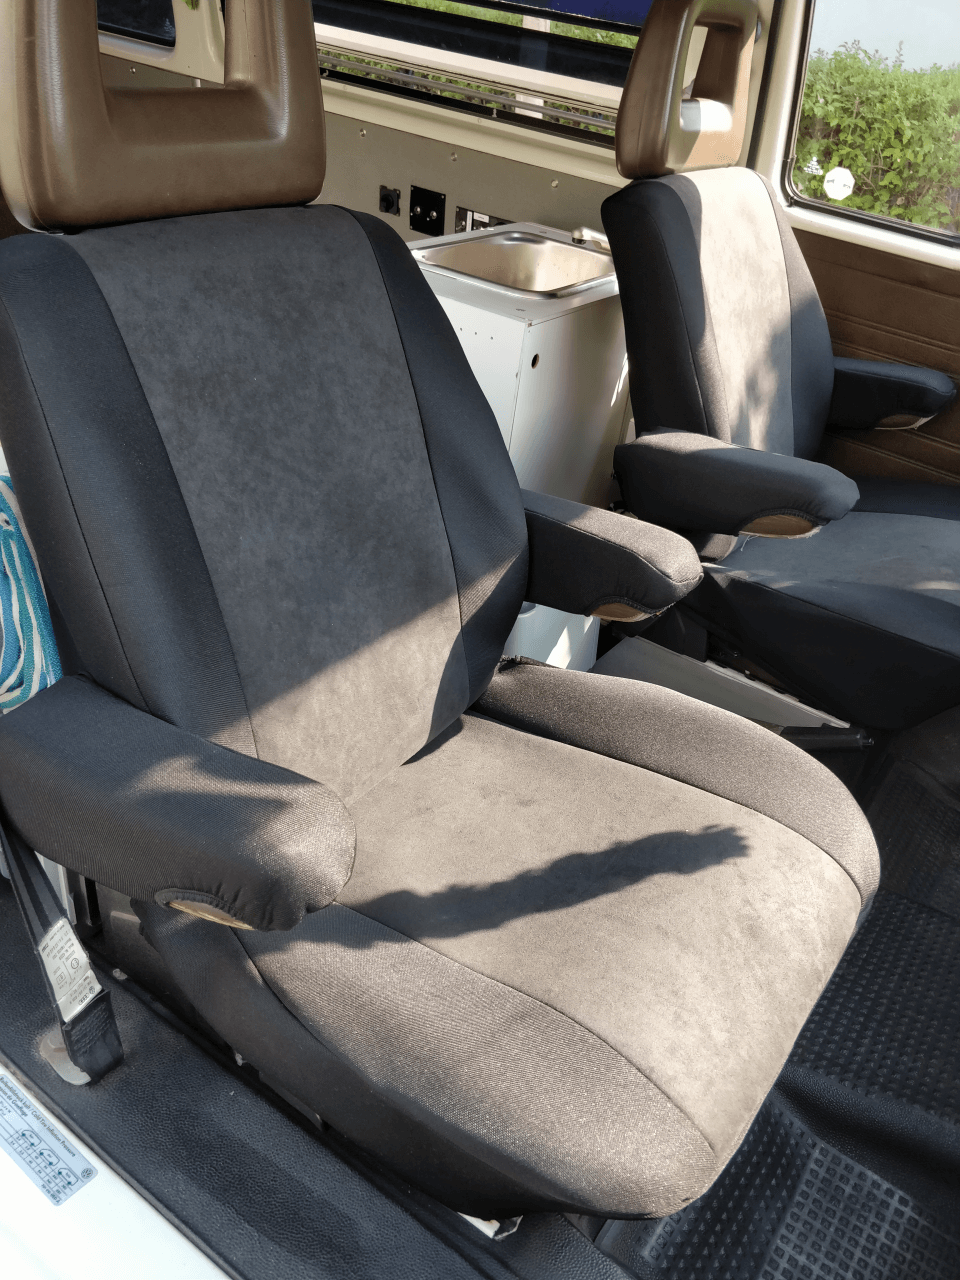
\includegraphics[width=0.4\textwidth, height=5cm, keepaspectratio]{../Bilder/Sylt/1.png}
    \caption{Neue Sitzbezüge}
  \end{centering}
\end{wrapfigure} 

Ein Geburtstag und eine damit verbundene Einladung lockte uns für einmal in den Norden.
Die Hitzewelle welche die Schweiz und Europa fest im Griff hatte liess uns von tieferen Temperaturen träumen.
Eine zweiwöchige Geschäftsreise nach Phoenix mit Spitzentemperaturen von 47°C erhöhten den Wunsch nach angenehmere Temperaturen nur noch mehr.
Das Ziel sollte Sylt sein.
Genauer gesagt Hörnum.
Da sich das Ziel doch über Tausend Kilometer entfernt befand, wurde aus einer Woche Ferien deren drei.
Eine Woche um in den Norden zu reisen, eine Woche auf Sylt und dann noch genügend Zeit um die Rückreise in den Süden anzutreten. 
Vor der Abfahrt sollte der Bus ein weiteres Mal für die lange Fahrt bereitgemacht werden.
Dieses Mal ging alles ganz fix.
Die neuen Sitzüberzüge passten wie angegossen und werten den Innenraum merklich auf.

\begin{figure}[hb]
    \centering
    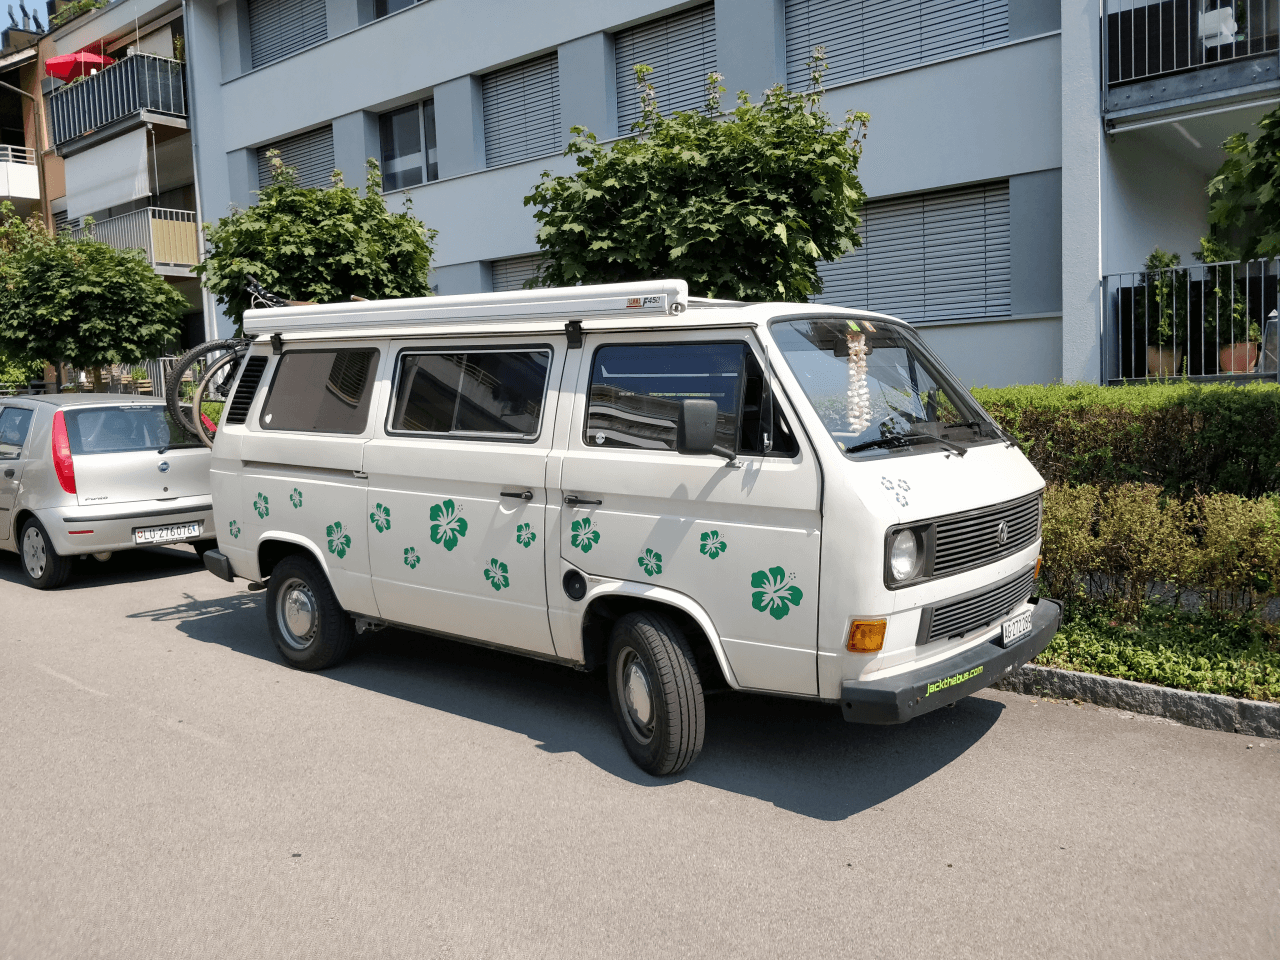
\includegraphics[width=\textwidth]{../Bilder/Sylt/2.png}
    \caption{Der Bus wieder einmal in Luzen}
    \label{img:Sylt}
\end{figure}

\newpage
\subsection{06.08.2018 Heisse Fahrt in den Norden} 
Eigentlich wollten wir schon am Samstag los. Ein Arzttermin (Grund für Arzttermin äusserst positiv) machte uns jedoch einen Strich durch die Rechnung.
Also ging die Fahrt erst am Montag kurz nach drei los.
Wie vorhin schon erwähnt war es ziemlich warm.
Die fehlende Klimaanlage machte sich relativ schnell bemerkbar und erzeugte bei der Beifahrerin nicht gerade Freude.
Das erste Ziel sollte Heidelberg sein.
Warum?
Einfach so, liegt auf der Strecke und sollte innerhalb eines halben Tages gut erreichbar sein.
Nebenbei scheint es auch eine hübsche Stadt zu sein. 
Die kurze Google Bildersuche schien auf jeden Fall darauf hinzuweisen.
Zu guter Letzt hat es dort Wasser im Form des Neckars, welche durch die Stadt fliesst.
Gerade bei den Temperaturen ein sehr gutes Argument.
Die Reise über Basel verlief problemlos und nur mit geringem Stau.
Zwischendurch meinte das Navi die Distanz zum Ziel zwar zu verringern, die Zeit bis zum Ziel jedoch stetig ansteigen zu lassen.
Nicht gerade motivierend.
Bis wir jedoch das Stauende erreicht hatten war das Schlimmste schon längst vorbei.
Unterwegs wurde Kontakt mit einem Zeltplatz aufgenommen und es wurde bestätigt, dass die Reception bis um halb Neun offen sein sollte.
Kurz vor Acht trafen wir dann auf dem Campingplatz ein.
Absolut durchnässt von den hohen Temperaturen war die Dusche eine reine Wohltat.
Der Campingplatz besitzt zwar ein kleines Restaurant, wir bevorzugten jedoch wieder einmal selbst zu kochen.
Vor der Abreise habe ich noch bei einem Italiener in Luzern feine Orecchiette und eine passende Sauce gekauft.
Danach hiess es dann bald einmal Licht aus im kleinen aber feinen VW Bus direkt am Neckar.

\begin{figure}[hb]
    \centering
    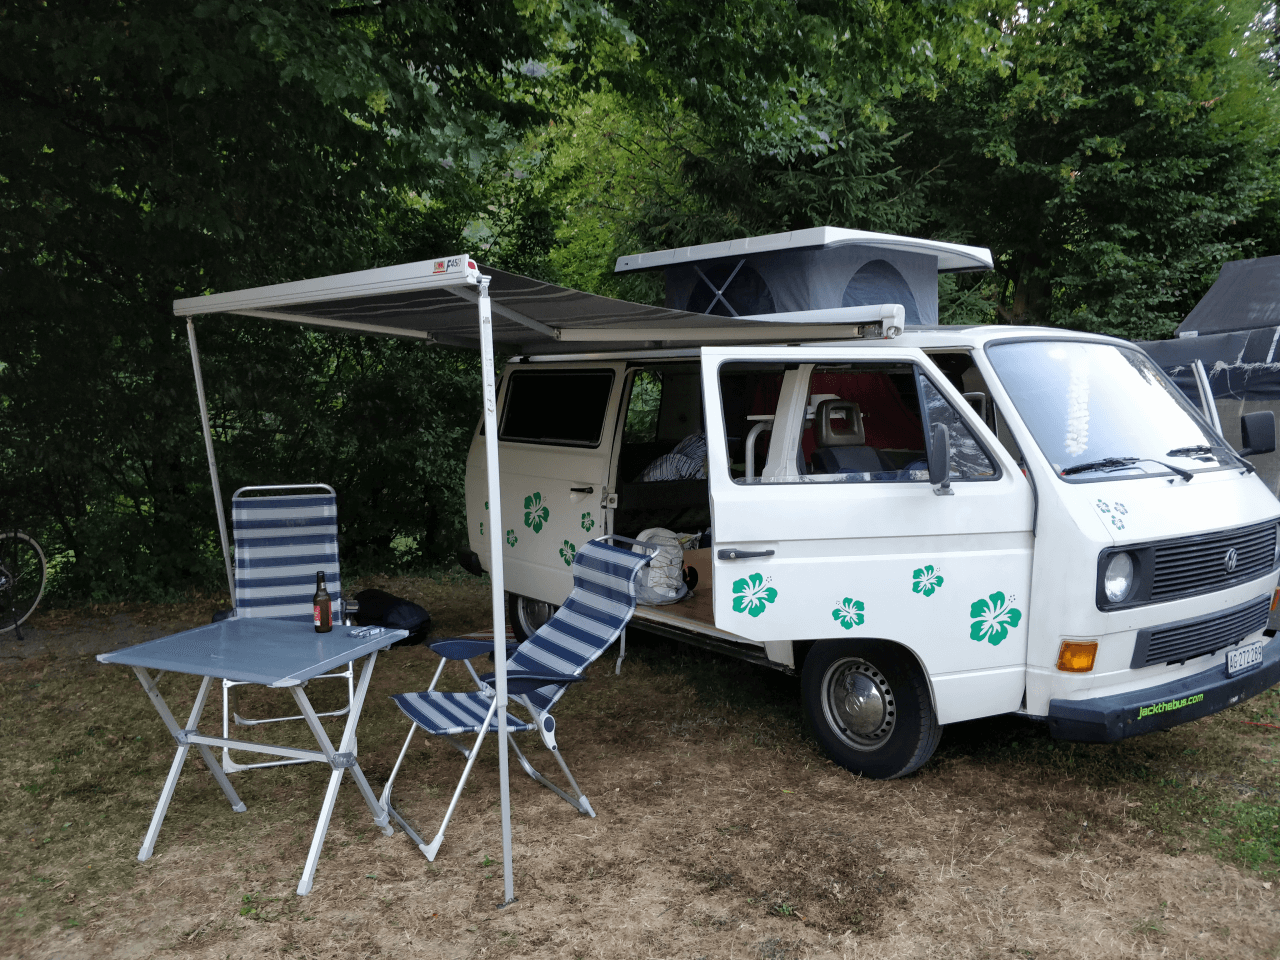
\includegraphics[width=\textwidth]{../Bilder/Sylt/3.png}
    \caption{Angekommen in Heidelberg}
    \label{img:Heidelberg_1}
\end{figure}

\subsection{07.08.2018 Zum Glück haben wir Fahrräder}
Endlich wieder einmal eine kühle Nacht.
Zuerst war es noch eher warm im Bus, darum wurde auf den Schlafsack verzichtet.
Mitten in der Nacht wurde es dann doch eher kühl, so dass der Schlafsack doch wieder eine Option wurde.
Wer hätte das gedacht.
Die am Vortag bestellten Plunder waren schon längst an der Kasse verfügbar als wir uns an das Frühstück machten.
Der Plan war die Stadt Heidelberg mit Hilfe der mitgebrachten Fahrräder zu erkunden. 
Google Maps sagte 40 Minuten für die paar Kilometer dem Fluss entlang vor.
Die Sonne wärmte schon wieder kräftig, als wir uns auf die Sättel schwangen und Richtung Stadt pedalierten.
Vorbei an etlichen Schleusen kam schon bald das Schloss in Sicht. 

\begin{figure}[H]
   \centering
      %\subfloat[CAPTION]{BILDERCODE}\qquad
   \subfloat{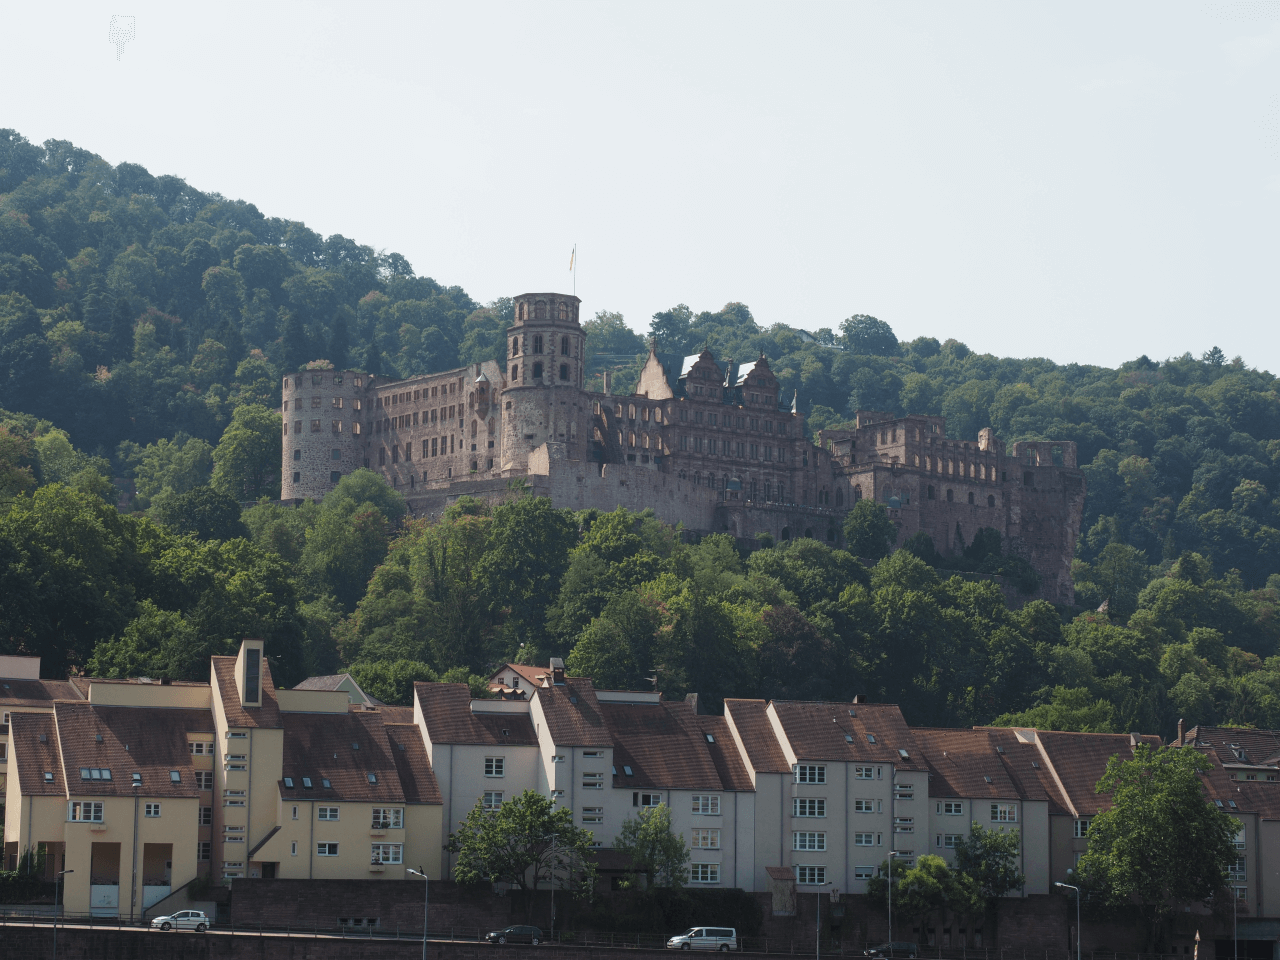
\includegraphics [width=0.3\textwidth]{../Bilder/Sylt/4.png}}\quad
   \subfloat{\includegraphics [width=0.3\textwidth]{../Bilder/Sylt/6.png}}\quad
   \subfloat{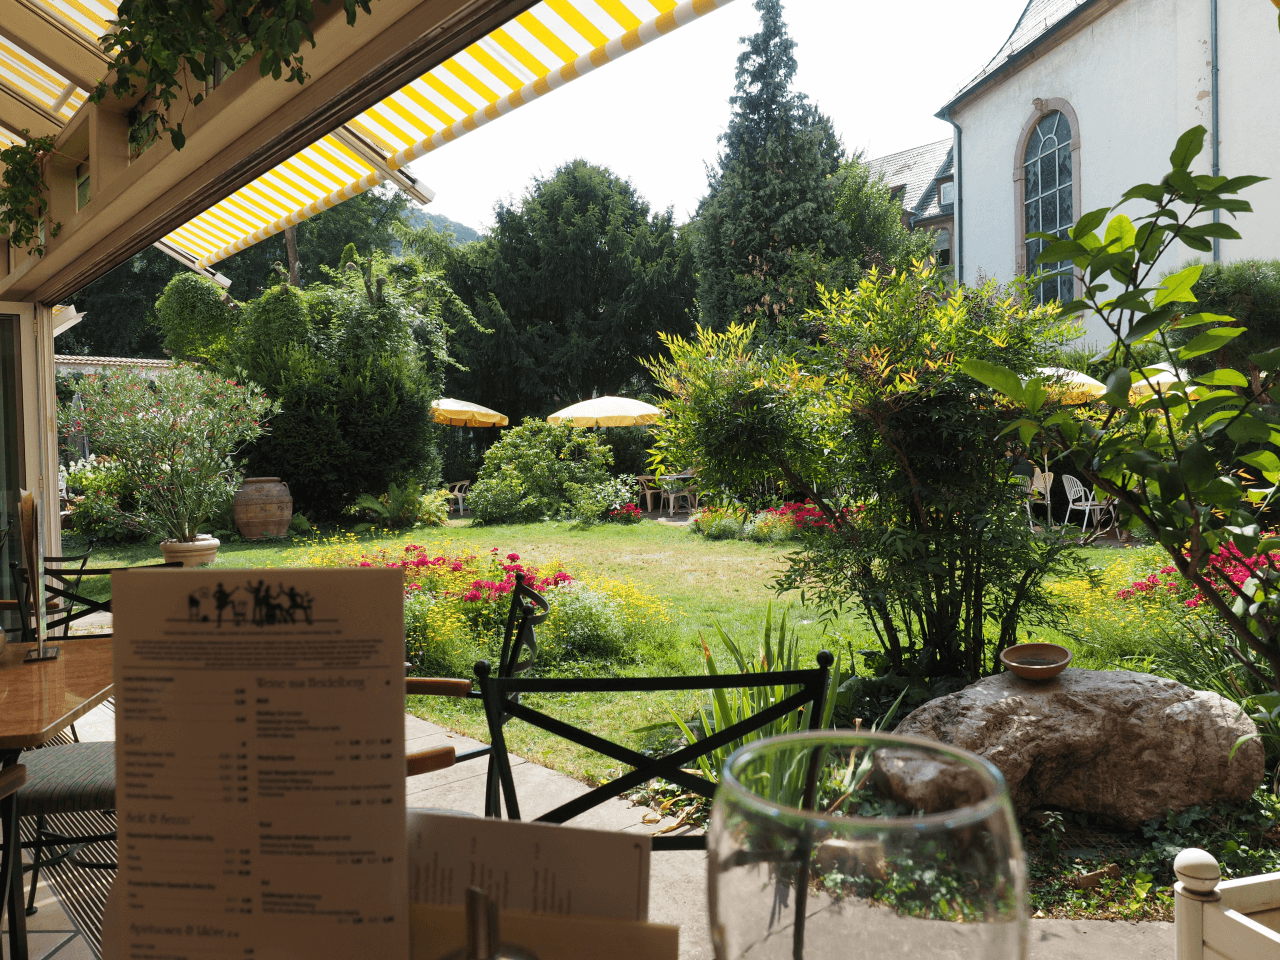
\includegraphics [width=0.3\textwidth]{../Bilder/Sylt/7.png}}\quad
   \caption[Heidelberg]{Heidelberg}
\end{figure}

Nachdem die Velos deponiert worden sind, ging es entlang der schier endlosen Fussgängerpromenade.
Ein Eis-Geschäft lockte uns in seine Fänge und nach einer gefühlten Ewigkeit ging es der Promenade entlang weiter.
Die sehr hohen Temperaturen führten dazu, dass der Weg wie ferngesteuert Richtung Wasser ging. 
Leider war die Strandbar am Nachmittag nicht offen. 
In einem Café wurde ein Salat zu sich genommen und bald darauf waren wir uns einig, dass es zurück zum Campingplatz gehen sollte um die Beine noch ein bisschen hochzulagern.
Ein Aldi auf dem Rückweg sorgte für neue Getränke und natürlich war der Durst und Hunger grösser als die verfügbaren Taschen.
So musste das Wasser auf dem Gepäckträger Platz finden. 
Nach der zweiten Bodenwelle verabschiedete sich das störrische Wasser Richtung Fluss und fiel die Böschung herunter.
Chantal pedalte unbeirrt weiter und liess sich auch vom hysterischen Rufen meinerseits nicht beirren.
Erst ein ganzes Stück später bemerkte sie das geparkte Velo und kehrte an den Tatort zurück, wo ich mich gerade mit 6 Flaschen bewaffnet wieder die Böschung hochkämpfte.
Da sich das Nachtessen vom Vortag bewährt hat, gab es noch einmal das selbe.
Während Chantal schon früh das Bett aufsuchte, gab ich mir noch Mühe und fing an die neuen Berichte zu schreiben.
Der nächste Tag sollte früh beginnen \dots

\subsection{08.08.2018 Wir machen Kilometer}
Die immer noch hohen Temperaturen motivierten früh aufzustehen und möglichst viele Kilometer in noch kühler Umgebung zu machen.
Das Problem dabei: Die Ruhezeiten auf dem Campingplatz.
Die Lösung wurde zusammen mit dem Kassier des Campingplatzes gefunden. Wir zügelten ganz einfach am Vorabend neben den Eingang / Ausgang des Platzes.
So würden wir hoffentlich nur einen kleinen Teil der Besucher wecken.
Um fünf Uhr wurden wir dann vom Wecker aus den Federn geholt und fingen an, alles in und an den Bus zu verräumen.
Um zwanzig vor sechs waren wir auf Achse und auf Ausschau nach einer Tankstelle, da der Tank schon sehr leer war.
Nach dem Tankstopp wurden kräftig Kilometer gemacht.
Erst ein weiterer Tankstopp mit Fahrerwechsel stoppte unser Fortschritt kurz.
Dann fingen die Warnungen wieder an. 
Nach Hannover staute sich der Verkehr um über eine Stunde.
Schnell war eine alternative Route gefunden, welcher wir folgten.
Vor dem Tagesziel Bremen verirrte sich dann Google Maps für ein Mal wahnsinnig. 
Dank sehr schlechten Mobilfunkverbindung konnte die Route nicht neu berechnet werden und wir wurden als Dank im Kreis herum geschickt.
Kurz nach halb zwei tauchte dann unser Ziel endlich auf.
Ein wunderschön gelegener Campingplatz zwischen Universität und dem Stadtwaldsee.
Die Eroberung und Erkundung von Bremen wurde auf den folgenden Tag verschoben und so wurde der See per pedes umrundet und beim Italiener direkt am See bei Sonnenuntergang eine Pizza genossen.
Nach spannender Lektüre über den Dalai Lama und einem Krimi der auf Sylt spielt gingen die Lichter im Bus aus.

\begin{figure}[H]
   \centering
      %\subfloat[CAPTION]{BILDERCODE}\qquad
   \subfloat{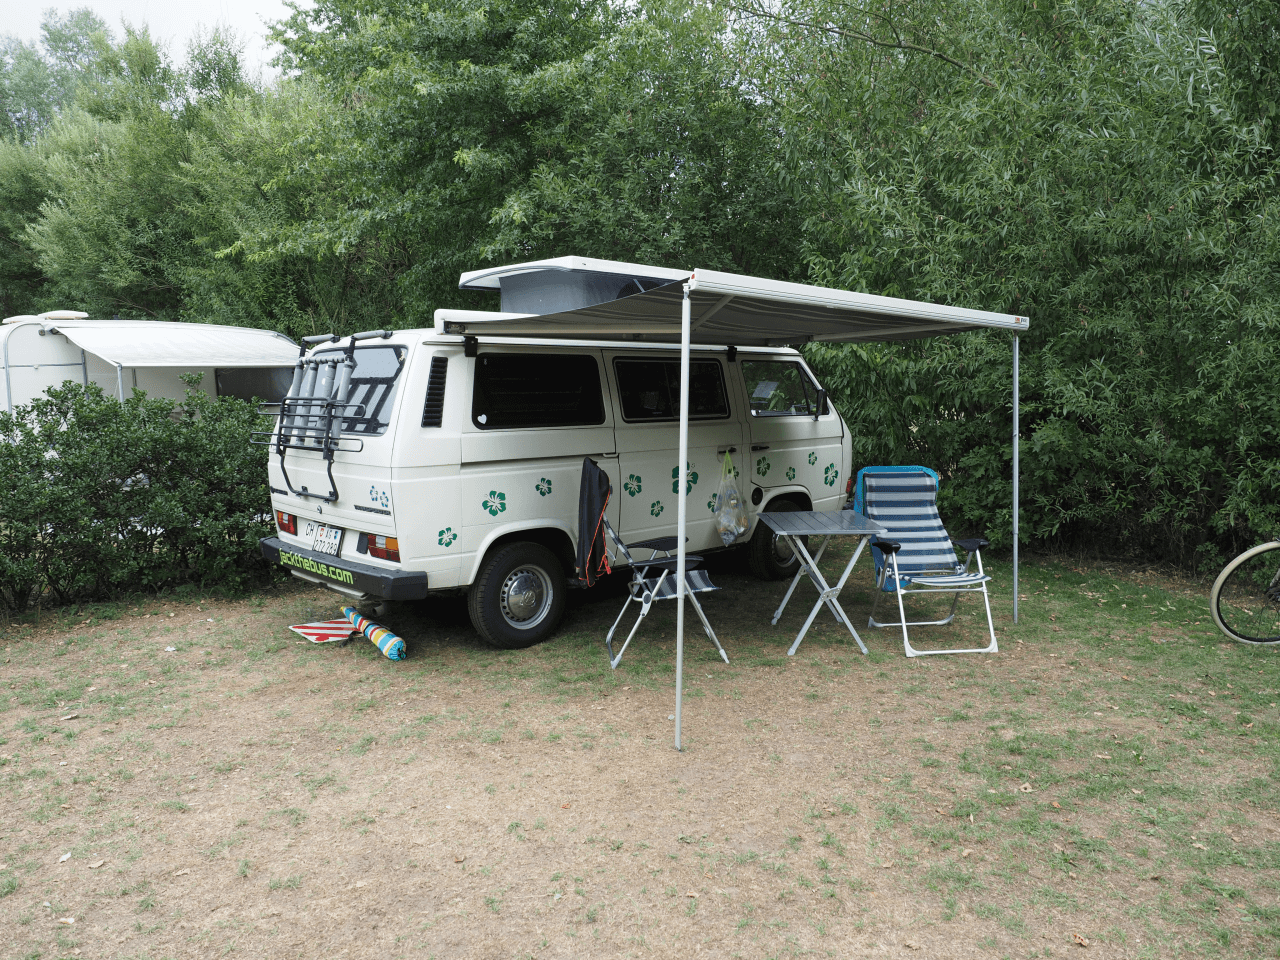
\includegraphics [width=0.3\textwidth]{../Bilder/Sylt/9.png}}\quad
   \subfloat{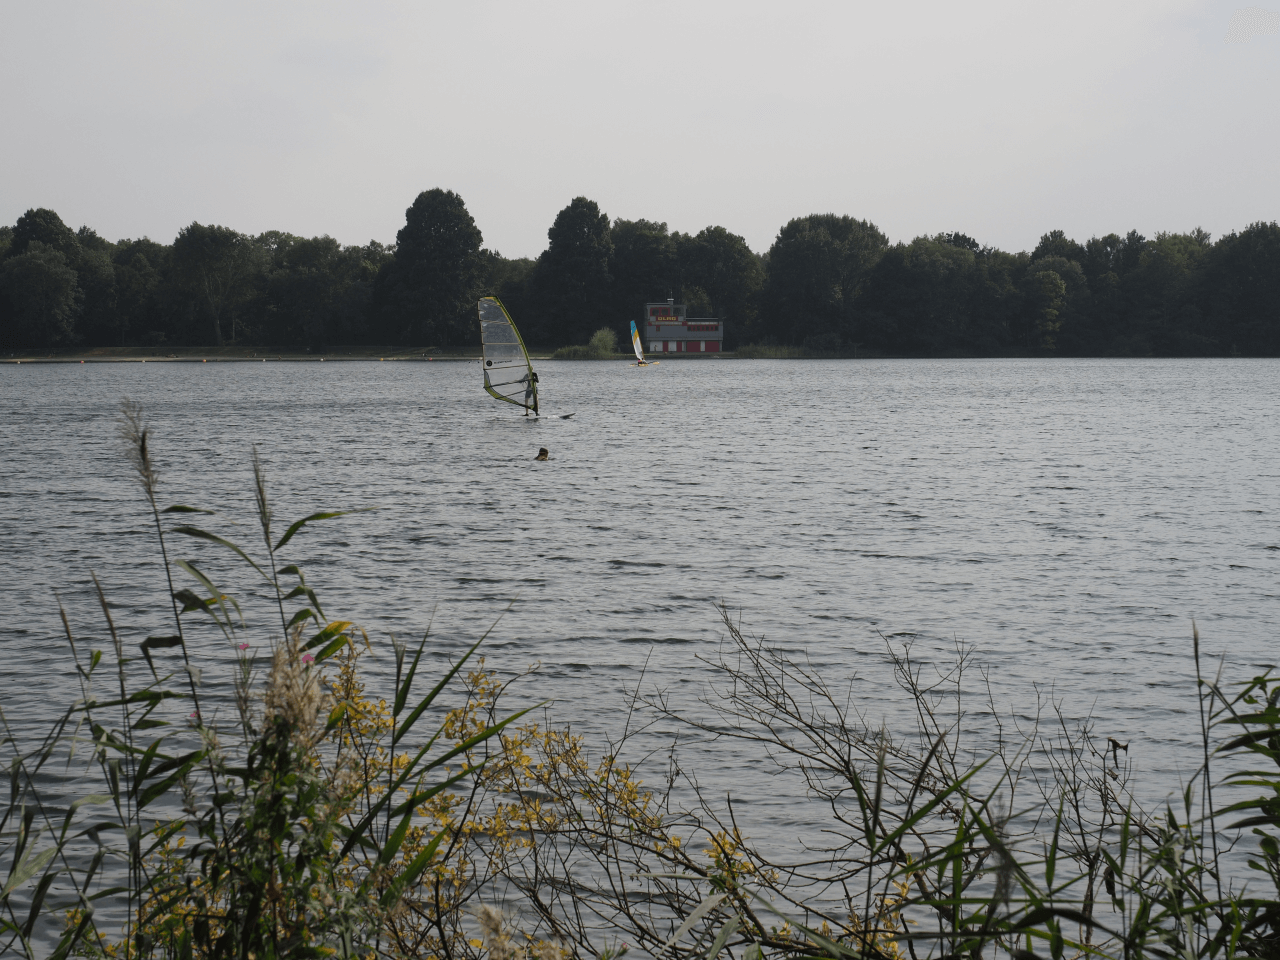
\includegraphics [width=0.3\textwidth]{../Bilder/Sylt/10.png}}\quad
   \subfloat{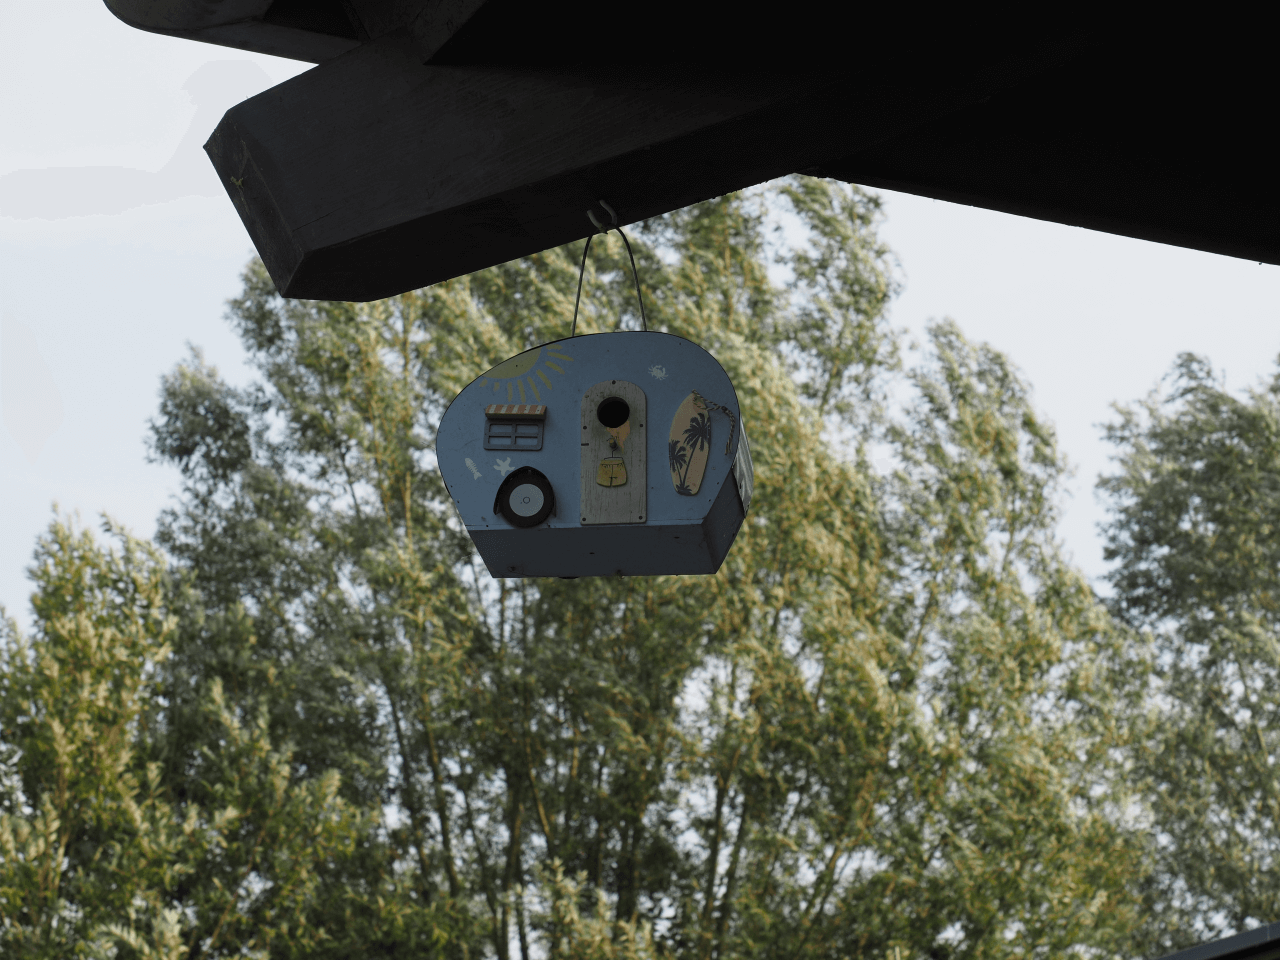
\includegraphics [width=0.3\textwidth]{../Bilder/Sylt/11.png}}\quad
   \caption[Campingplatz in Bremen]{Campingplatz in Bremen}
\end{figure}

\subsection{09.08.2018 Bremen oder doch eher Kopenhagen}
Um positiv überrascht zu werden hilft es am meisten keine Erwartungen zu haben.
Ich / wir hatten überhaupt keine Erwartungen an Bremen.
Das einzige was mit in den Sinn kam, waren die Bremer Stadtmusikanten.
So ging es nach einem Frühstück und einem kurzen Besuch des Universum der Universität Bremen mit dem Fahrrad Richtung Innenstadt.

\begin{figure}[H]
   \centering
      %\subfloat[CAPTION]{BILDERCODE}\qquad
   \subfloat{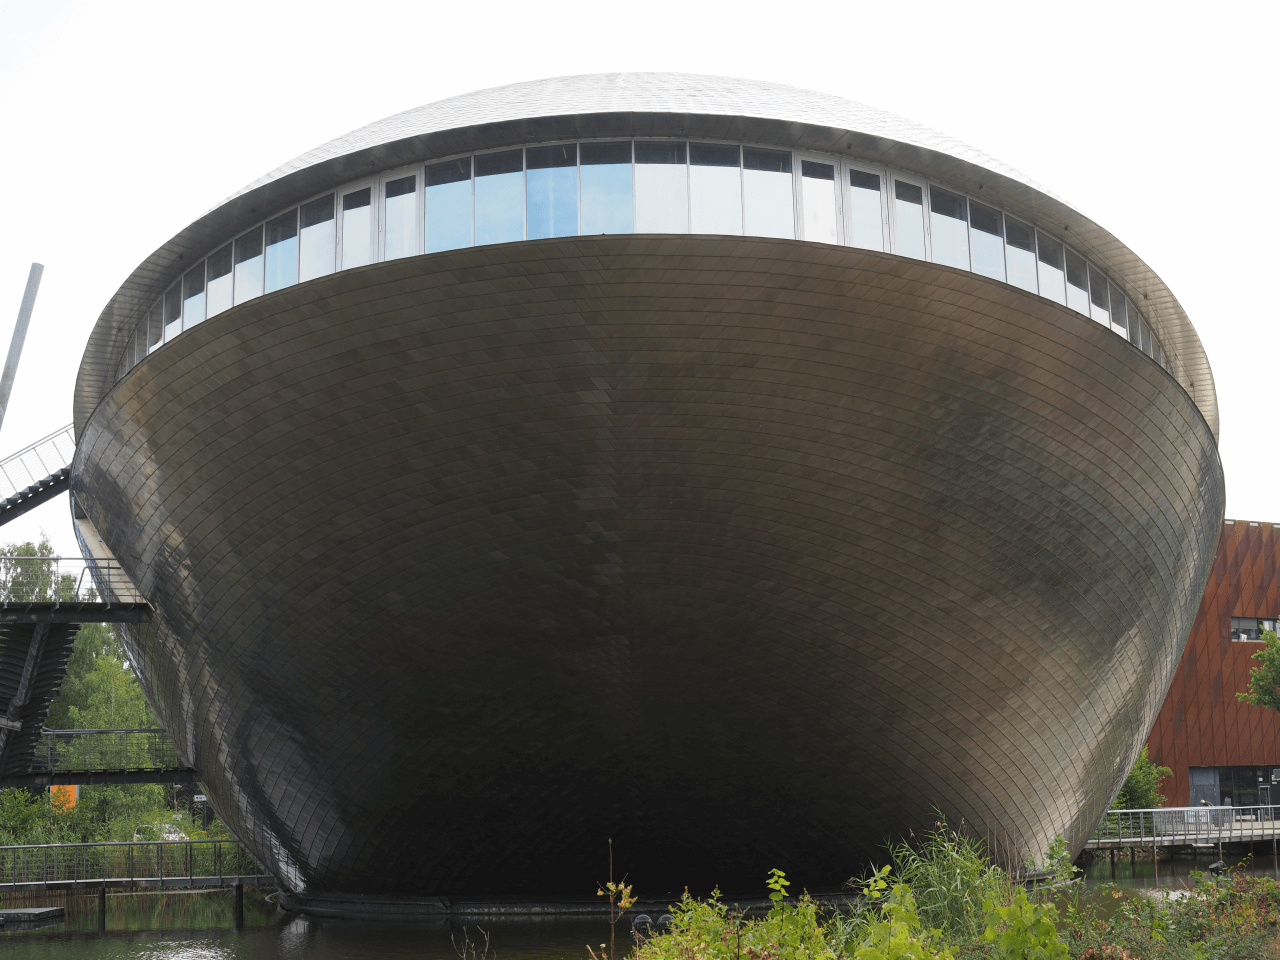
\includegraphics [width=0.45\textwidth]{../Bilder/Sylt/13.png}}\quad
   \subfloat{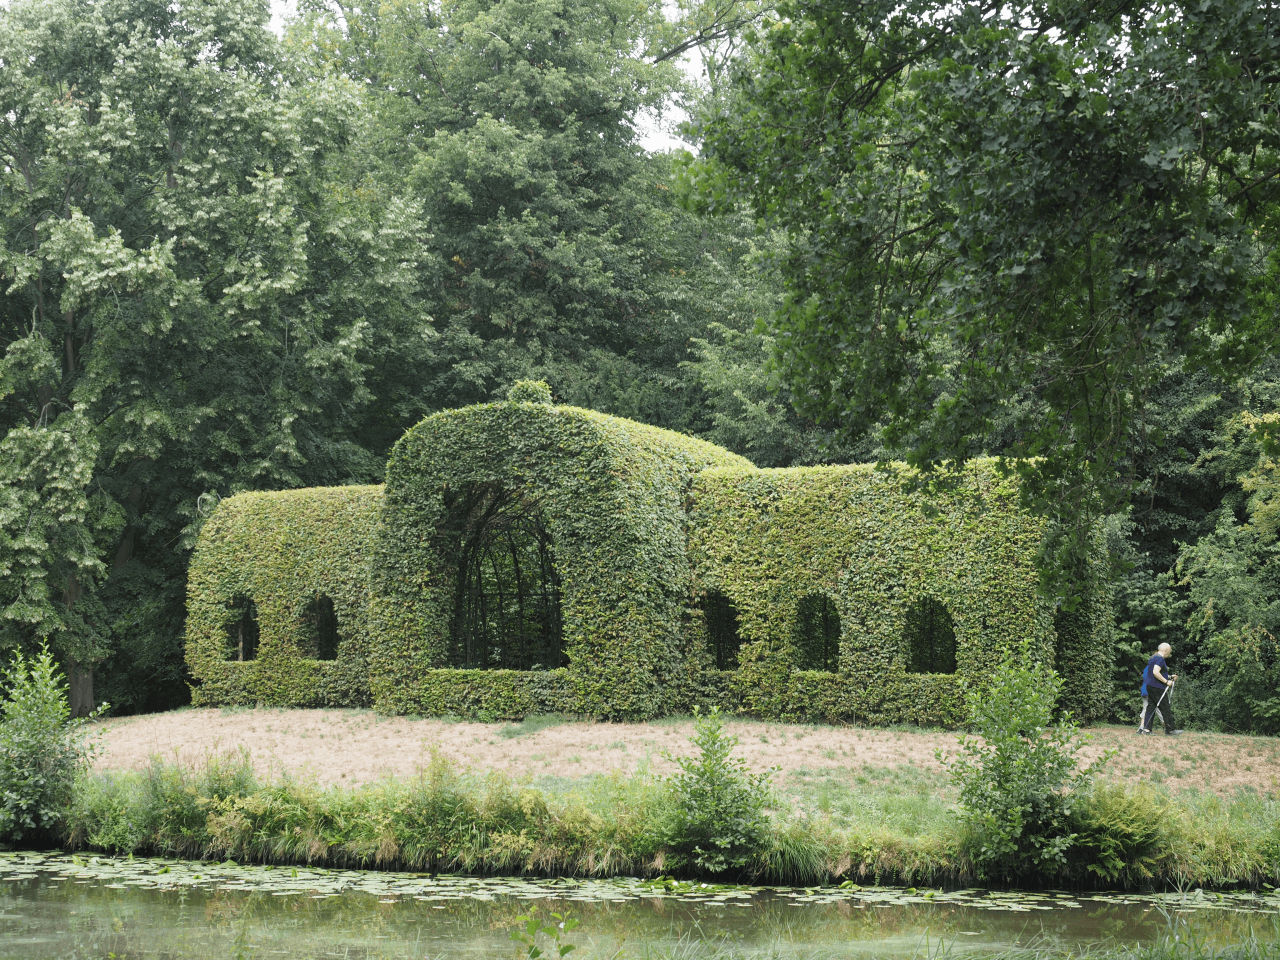
\includegraphics [width=0.5\textwidth]{../Bilder/Sylt/14.png}}\quad
   \caption[Universum und Bürgerpark]{Universum und Bürgerpark}
\end{figure}

Der Weg dorthin war wunderschön in einem Park gelegen und wenn wir den Park verlassen mussten, war da sicher ein Fahrradweg zu Verfügung.
Die ganze Stadt scheint sehr fahrradfreundlich ausgerichtet zu sein.
Wo man hinkommt hat der Fahrradfahrer Vortritt, sind extra Fahrradstreifen vorhanden oder es werden ganze Strassen zu Fahrradstrassen erklärt auf denen die Autos nur noch geduldet werden.
In der Innenstadt angekommen, sind uns sofort die Marktstände mit Fressalien aufgefallen. Leider wurden diese fahrlässig links liegen gelassen.
Die Böttcherstrasse war unser erstes Ziel. Beeindruckend die Ansammlung von alten, gut erhaltenen Häuser.

\begin{figure}[t]
   \centering
      %\subfloat[CAPTION]{BILDERCODE}\qquad
   \subfloat{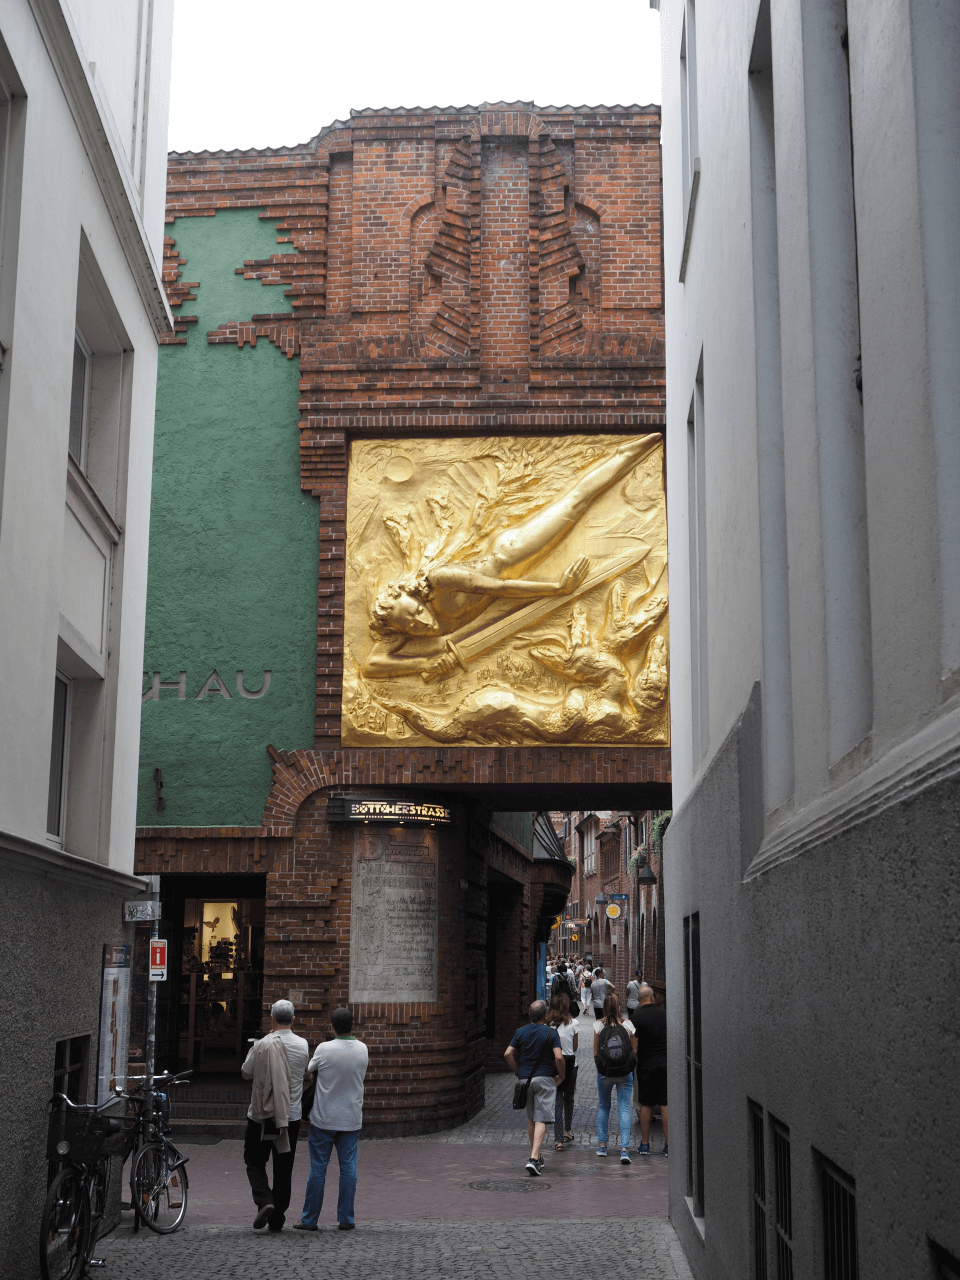
\includegraphics [width=0.3\textwidth]{../Bilder/Sylt/15.png}}\quad
   \subfloat{\includegraphics [width=0.3\textwidth]{../Bilder/Sylt/19.png}}\quad
   \subfloat{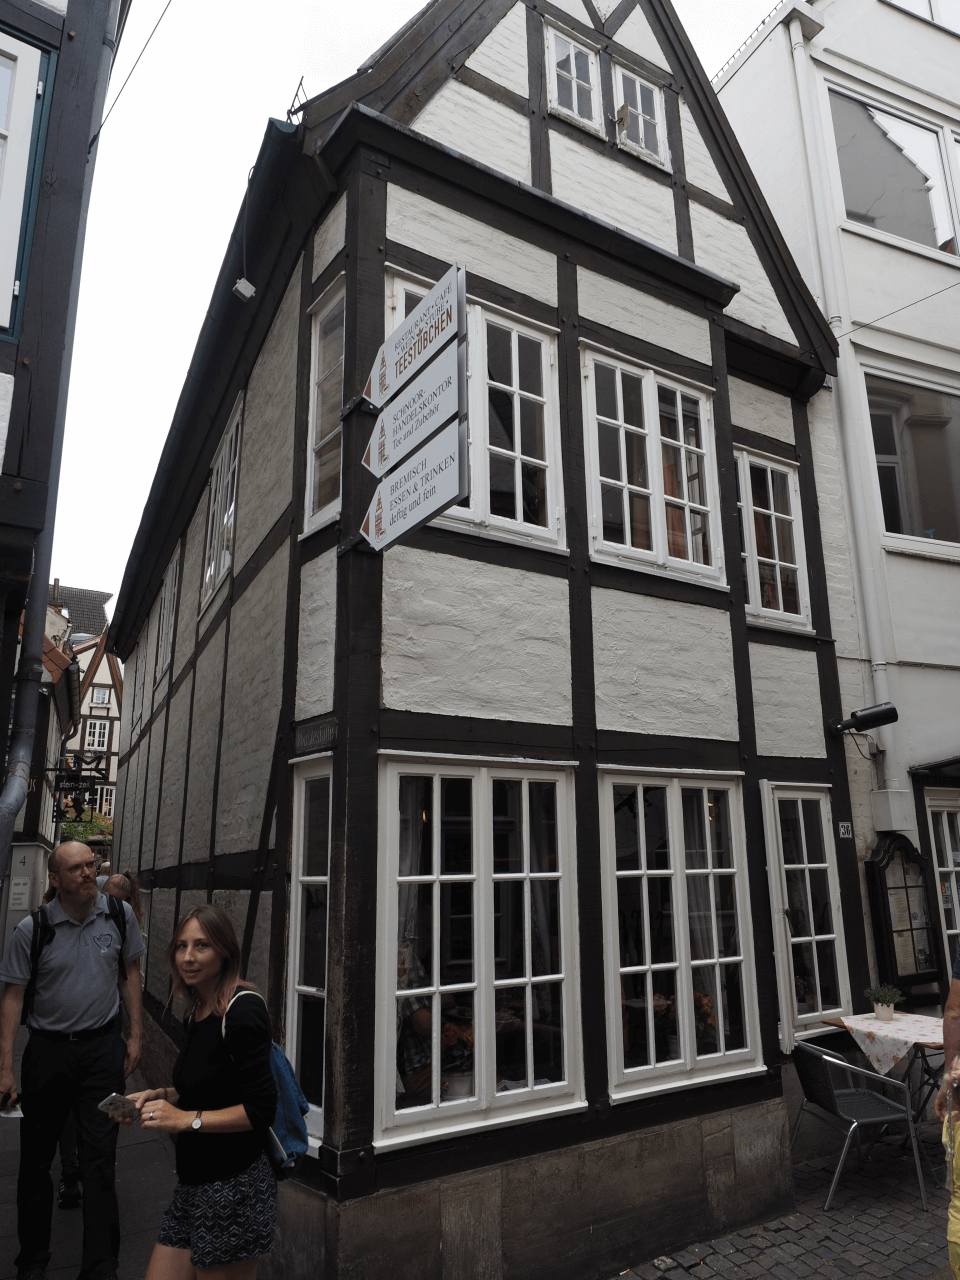
\includegraphics [width=0.3\textwidth]{../Bilder/Sylt/25.png}}\quad
   \caption[Böttcherstrasse und Schnorr-Viertel]{Böttcherstrasse und Schnorr-Viertel}
\end{figure}


\begin{wrapfigure}{R}{0.45\textwidth} 
  \begin{centering}
    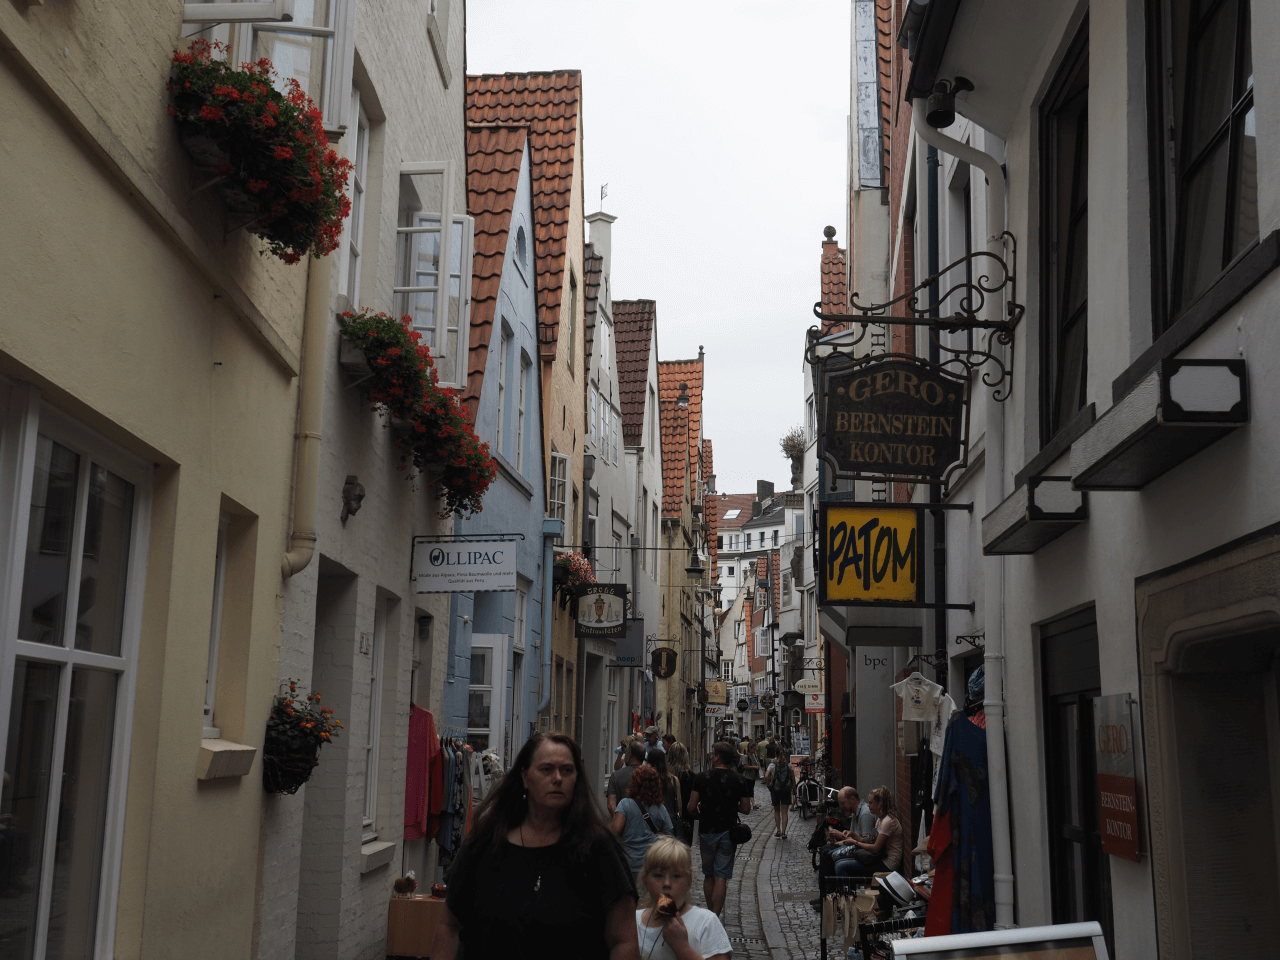
\includegraphics[width=0.4\textwidth, height=5cm, keepaspectratio]{../Bilder/Sylt/21.png}
    \caption{Schnorr-Viertel}
  \end{centering}
\end{wrapfigure} 

Danach ohne Unterbruch in das Schnorr-Viertel.
Eine sehr gute Gelegenheit für Chantal die trendigen Geschäfte zu erkunden.
Der Magen verlangte nach einer Pause. 
Frikadelle, Bratkartoffel und Rotkraut warteten auf uns.
Chantal fand neben neben den Imbissbuden einen super healthy veganen Stand der Porridge anbot.
Einen Moment später öffnete der Himmel die Schleussen und motivierte uns nicht gerade für die Heimkehr mit den Velos.
Aus wettertechnischen Gründen besuchten wir noch ein Geschäft, in dem ich einen genialen Hefter kaufte. 
Dies unter blöden Sprüchen meiner besseren Hälfte.
Die Rückfahrt durch den Park konnten wir wieder bei schönstem Wetter antreten.
Ich ging noch kurz unsere Wasservorräte aufstocken und als ich zurückkam und eine Dusche genoss verdunkelte sich der Himmel.
Nervöse Aktivitäten auf dem Campingplatz kündigten das aufkommende schlechte Wetter an.
Wir konnten gerade noch unsere sieben Sachen, die Markise und das Dach einziehen bevor es richtig losging.
Es seichte sprichwörtlich horizontal.
Nach dem überstandenen Sturm wagten wir den kurzen Weg in die Pizzeria.
Der vorbeigezogene Sturm führte zu einem vollen Innenraum, wir wagten jedoch den Versuch und setzten uns nach draussen.
\newpage
\subsection{10.08.2018 Die letzte Etappe}

\begin{wrapfigure}{L}{0.35\textwidth} 
  \begin{centering}
    \includegraphics[width=0.4\textwidth, height=5cm, keepaspectratio]{../Bilder/Sylt/34.png}
    \caption{Leuchtturm von Hörnum}
  \end{centering}
\end{wrapfigure} 

Heute wurde ausgeschlafen.
Danach genossen wir ein Frühstück and der erfrischend kühlen Morgenluft.
Ein weiteres Mal packten wir alles in den Bus und machten uns auf, das letzte Teilstück nach Sylt unter die Räder zu nehmen.
Kurz vor Elf Uhr waren wir unterwegs Richtung Hamburg, durch den Elbtunnel und weiter alles Richtung Flensburg oder grob gesagt Norden.
Nach dem wir die Autobahn verlassen hatten, mussten Mensch und Maschine dringend betankt werden.
So einfach gar nicht auf diesem Teilstück.
Wir mussten dann die Hauptstrasse verlassen, um irgendwie an Sprit zu kommen.
Bei der ersten Tankstelle funktionierte dann die EC Karte, wie auch die Visa nicht.
Glücklicherweise war keine 100 Meter entfernt eine zweite.
Diese leider ohne Restaurant.
So ging die Fahrt dank Benzin zwar weiter, die Magen knurrten jedoch noch immer.
Ein Rastplatz tauchte dann doch noch auf und der Blinker wurde gestellt.
Ein älterer Herr mit Gips eine Frau und ihr Sohn waren die einzigen Gäste.
Nach zwei riesen Currywürste fragte uns der \glqq Wirt\grqq{} wohin wir denn unterwegs sind.
Nach unserer Antwort meinte er nur kühl: \glqq Was wollt ihr dort? Geht nach Dänemark, ist schöner und günstiger\grqq{}
Nach dem erfahren hat das wir aus der Schweiz sind, kam wie aus der Pistole geschossen: \glqq Aus der Schweiz? Ihr habt genug Geld, geht nach Sylt.\grqq{}
Ein nervöser Rolls-Royce Fahrer vor uns sorgte dann für eine Lachnummer.
Ein kurzer Stau sorgte für einen erhöhten Blutdruck des Fahrers mit dem edle Gerät.
Mit allen Mitteln wurde versucht sich an den stauenden Autos vorbeizudrängeln. 
Ein Abzweiger versprach eine Möglichkeit den Stau zu umfahren.
Dass wurde sofort von meinem neuen Lieblingsfahrer in die Tat umgesetzt,
Zehn Minuten später tauchte das Edel-Gefährt wieder von links auf. 
Er musste sich dann jedoch deutlich hinter uns einordnen.
Bei der Ankunft bei der Bahn, für die Überfahrt nach Sylt hatten wir ein weiteres Mal grosses Glück.
Ein blauer Zug sollte sofort fahren.
Die Überfahrt, notabene Dank der Höhe des Buses Rückwärts, verlief problemlos.
Einzig eine laut Aussage der Bahn völlig überraschend kreuzender Zug zwang uns zu einer Pause.
Die kurze letzte Fahrt in den Süden der Insel bezwang der Bus mit bravour.
Wir hatten das Ziel Sylt nach 1300km problemlos erreicht.
Jetzt sollte der Bus zuerst einmal Pause machen, bevor wir dann in einer Woche den Rückweg in die Schweiz antreten werden.

\begin{figure}[b]
   \centering
      %\subfloat[CAPTION]{BILDERCODE}\qquad
   \subfloat{\includegraphics [width=0.3\textwidth]{../Bilder/Sylt/31.png}}\quad
   \subfloat{\includegraphics [width=0.3\textwidth]{../Bilder/Sylt/33.png}}\quad
   \subfloat{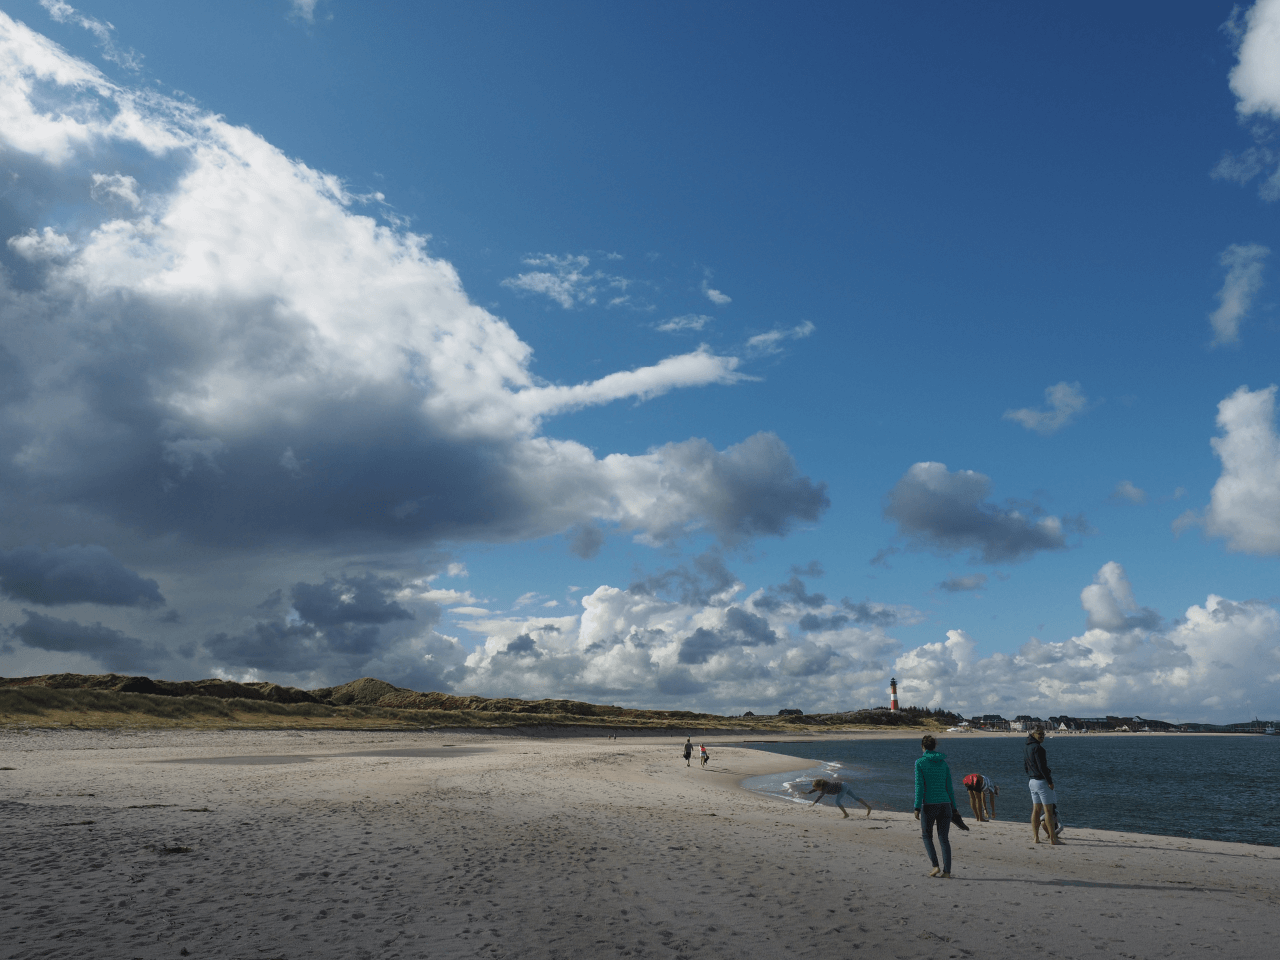
\includegraphics [width=0.3\textwidth]{../Bilder/Sylt/35.png}}\quad
   \caption[Sylt]{Sylt}
\end{figure}

\subsection{11. - 17.08.2018 Ferien auf Sylt}
Wie haben eine wunderschöne Woche auf Sylt verbracht.

\begin{itemize}
\item Sehr viel gegessen: Matjesbrötchen, Krabbenbrötchen, Muscheln und Apfelstrudel.
\item Noch mehr getrunken: Tote Tante Bier und Wein.
\item Sehr viel erlebt: Wandern in den Dünen, Wattwanderung von der Insel Anrum zur Insel Föhr. Strandchorbsitzen, Fussball spielen am Strand \dots 
\end{itemize} 

\begin{center}
\textbf{Vielen Dank an Mirjam und Vik für die gute Idee und die Rundumversorgung.} 
\end{center}

Ein paar Impressionen der Woche:

\begin{figure}[H]
   \centering
      %\subfloat[CAPTION]{BILDERCODE}\qquad
   \subfloat{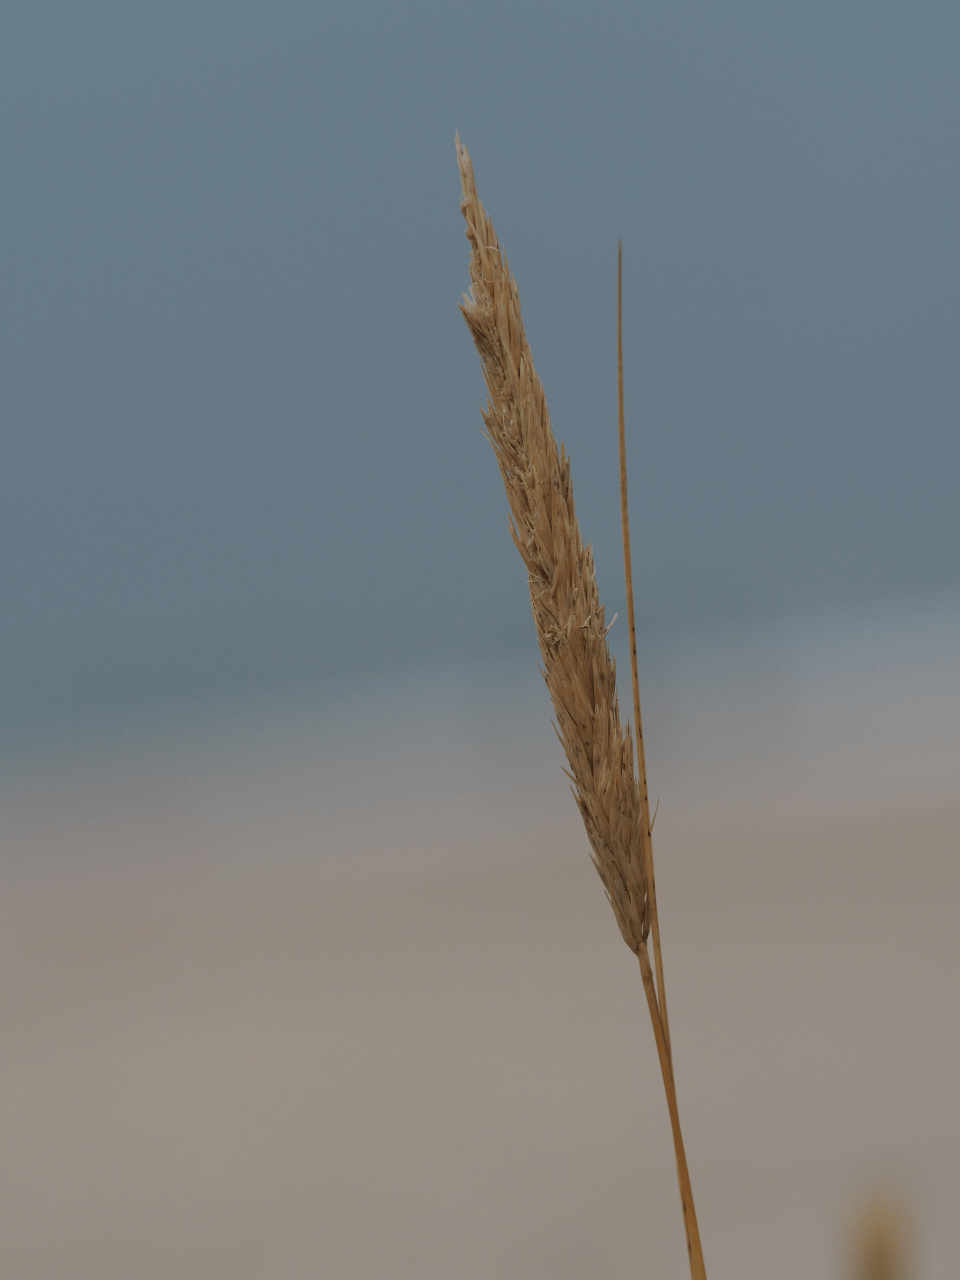
\includegraphics [width=0.45\textwidth]{../Bilder/Sylt/37.png}}\quad
   \subfloat{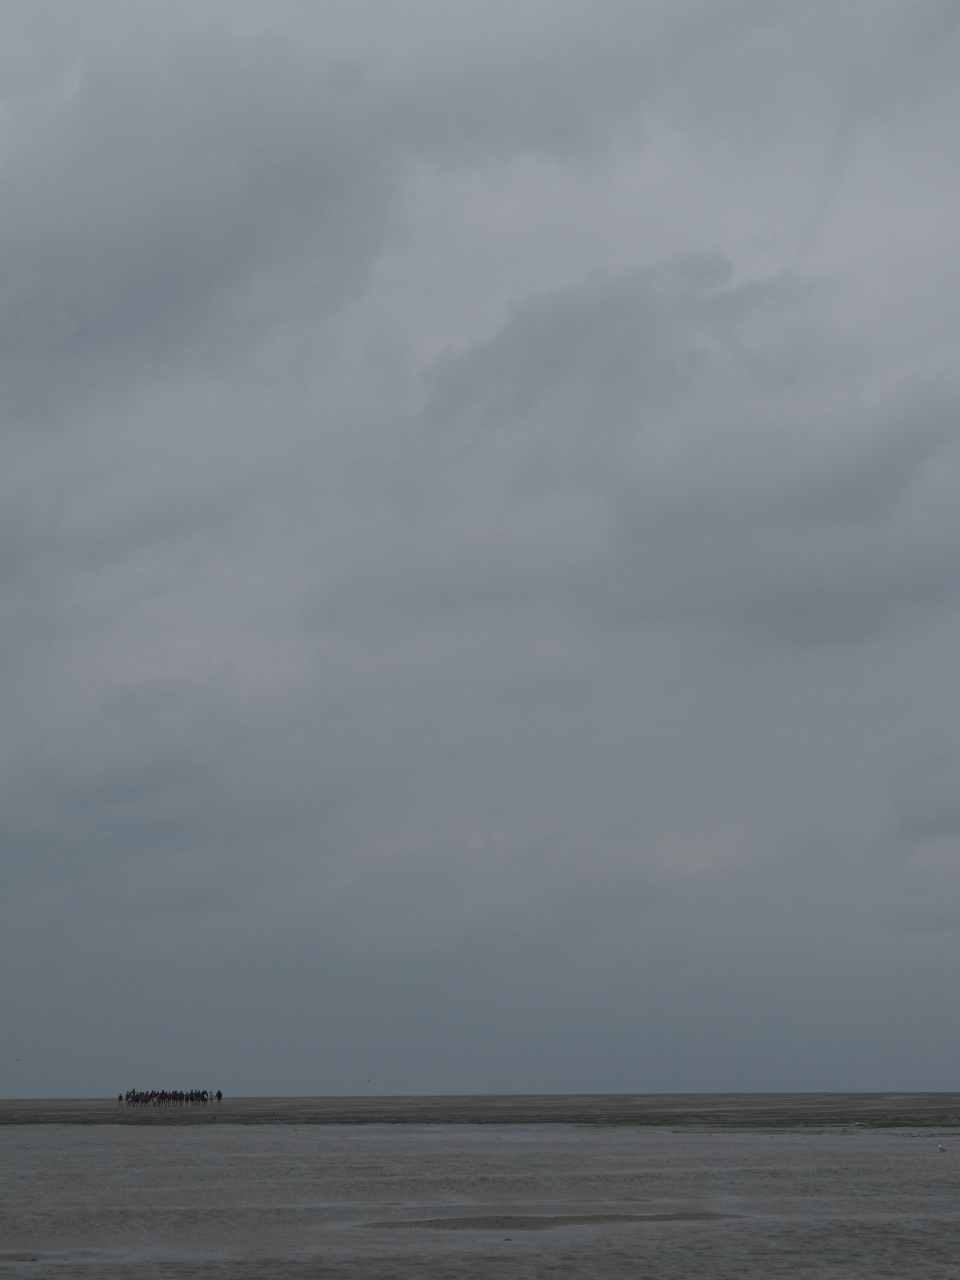
\includegraphics [width=0.45\textwidth]{../Bilder/Sylt/41.png}}\quad
   \caption[Wunderschöne Strände]{Wunderschöne Strände}
\end{figure}

\begin{figure}[H]
   \centering
      %\subfloat[CAPTION]{BILDERCODE}\qquad
   \subfloat{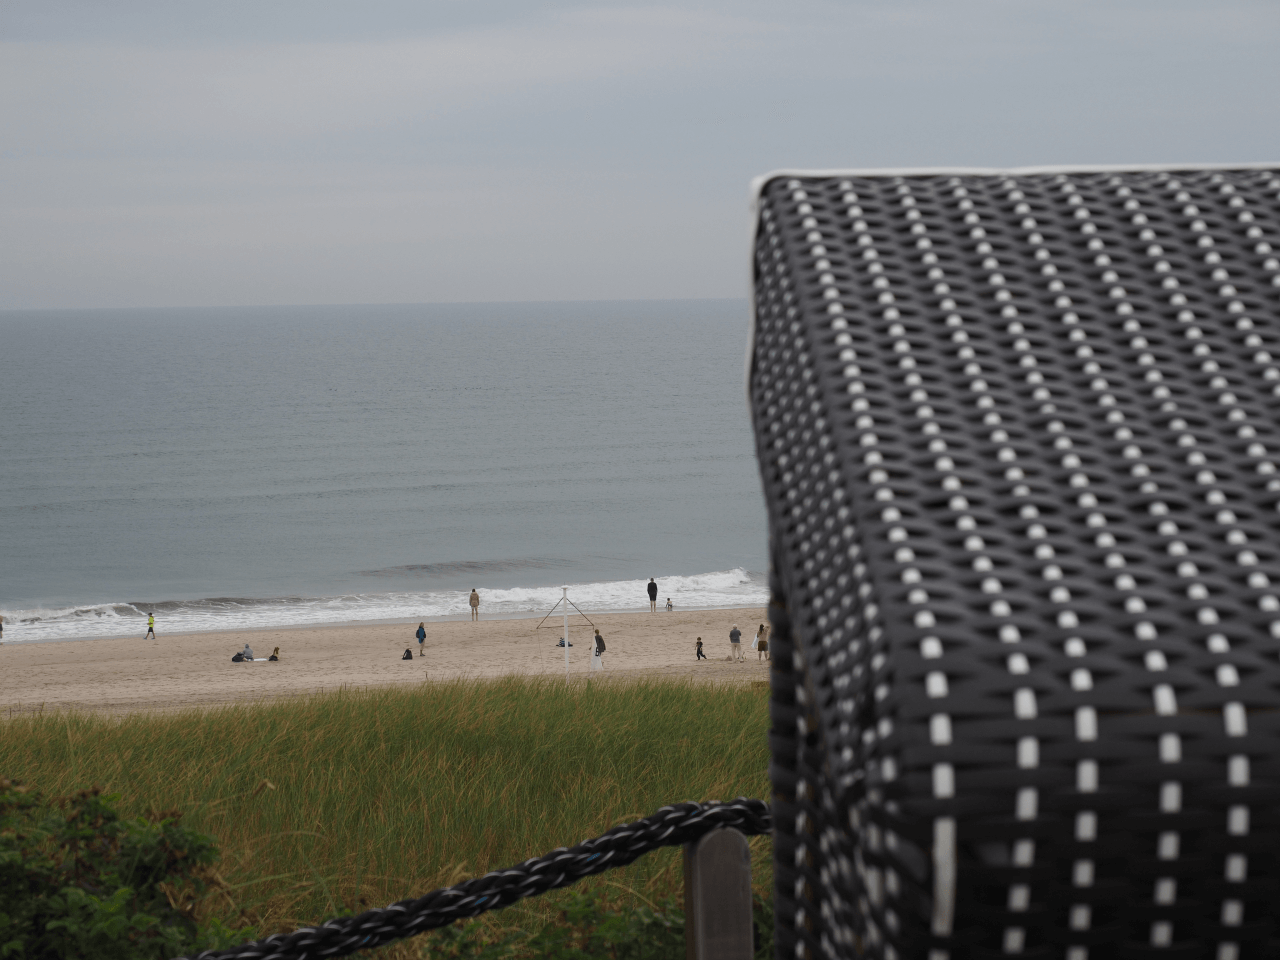
\includegraphics [width=0.3\textwidth]{../Bilder/Sylt/36.png}}\quad
   \subfloat{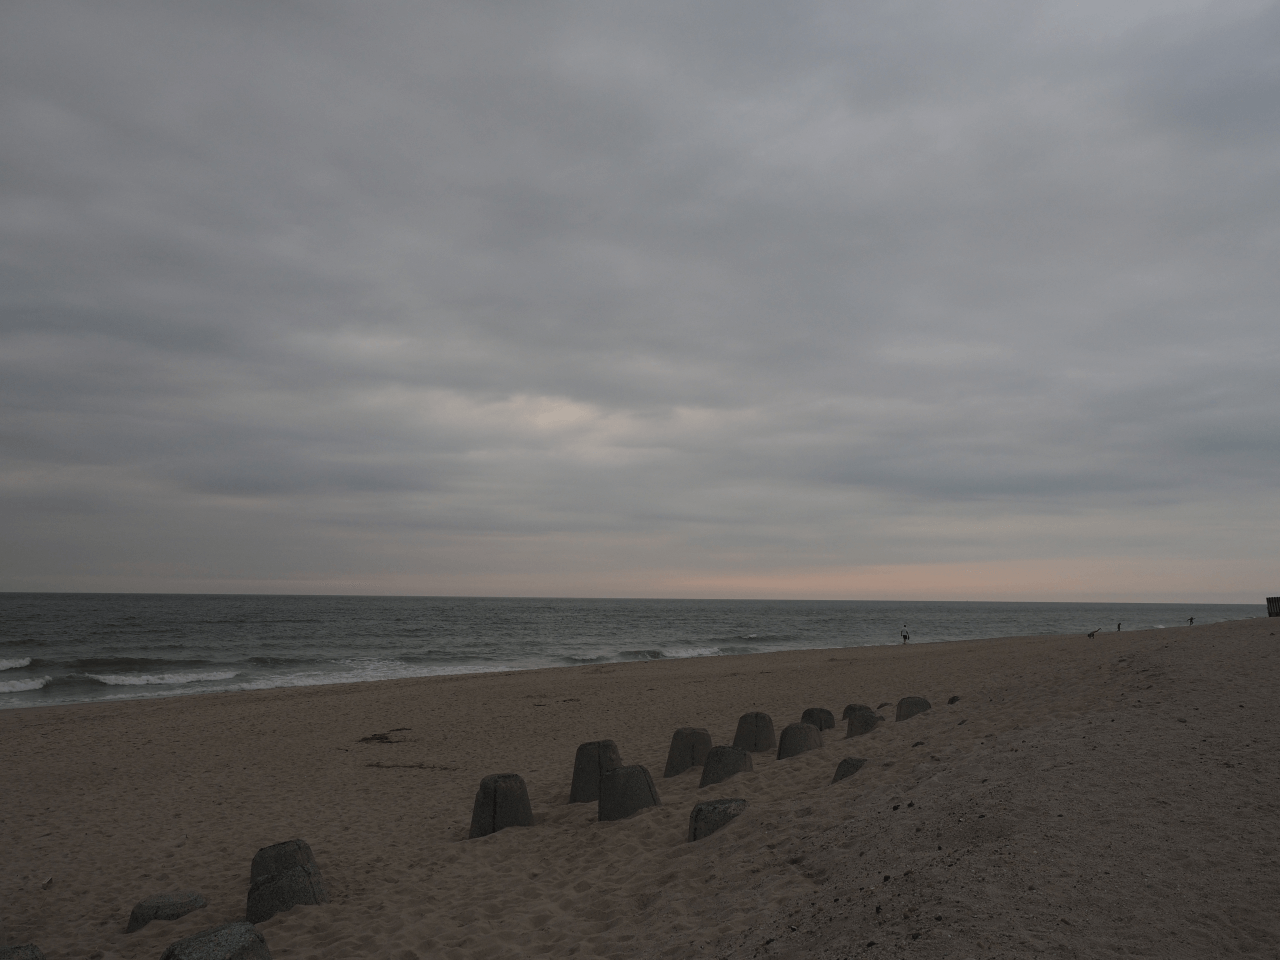
\includegraphics [width=0.3\textwidth]{../Bilder/Sylt/40.png}}\quad
   \subfloat{\includegraphics [width=0.3\textwidth]{../Bilder/Sylt/42.png}}\quad
   \caption[Typisch Sylt]{Typisch Sylt}
\end{figure}
\newpage

\subsection{18.08.2018 Es geht wieder Richtung Süden}

\begin{wrapfigure}{L}{0.45\textwidth} 
  \begin{centering}
    \includegraphics[width=0.4\textwidth, height=5cm, keepaspectratio]{../Bilder/Sylt/43.png}
    \caption{Überfahrt zurück auf das Festland}
  \end{centering}
\end{wrapfigure} 

Schon am Vorabend wuselten alle durch das grosse Weisse Haus.
(Glücklicherweise nicht dasselbe in dem auch der grosse orange Affe wohnt.)
Alle waren mit Packen beschäftigt.
Nach einer kurzen Nacht wurden wir unsanft um 4:00 Uhr in der Nacht geweckt.
Der erste verfügbare Zug sollte uns wieder auf das Festland bringen.
Schon um diese Zeit gab es einen kleinen Stau rund um Westerland und die Verladestation.
Schon hier trennten sich unsere Wege, Chantal musste am Montag wieder im Büro sein, ich hatte noch eine Woche Gnadenzeit.
Mein erstes Ziel nach Sylt sollte Wolfsburg sein, warum?
Keine Ahnung, liegt mehr oder weniger auf der Strecke und ist ja so eine Art Geburtstätte des Buses.
Die Autostadt sollte also besichtigt werden.
Ein paar Hundert Kilometer waren jedoch noch zurückzulegen.
In Uelzen wurde ich durch eine Schleuse abgelenkt und machte eine kurze Pause um mir die Beine zu vertreten.

\begin{figure}[h]
    \centering
    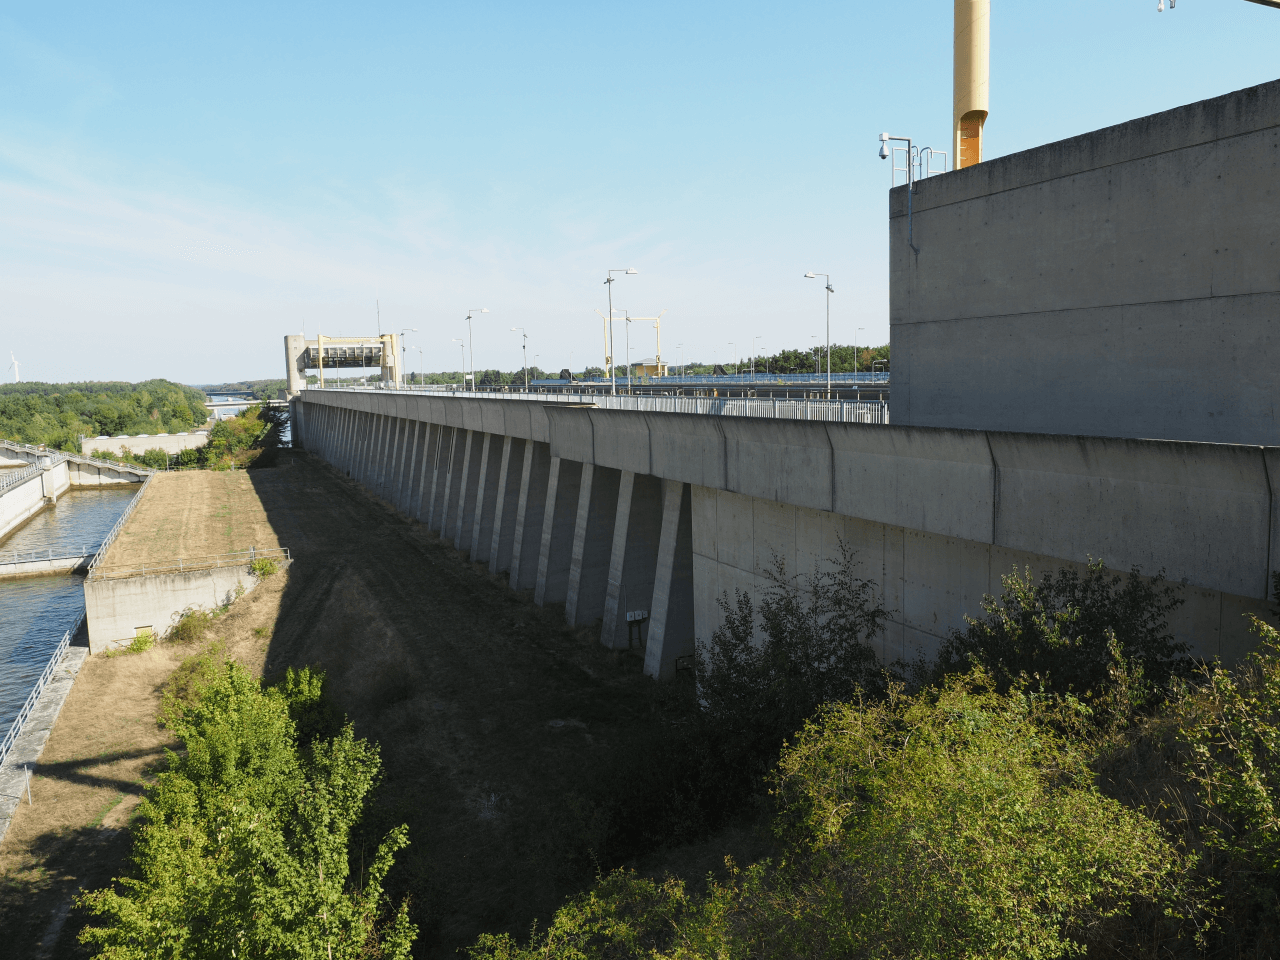
\includegraphics[width=\textwidth]{../Bilder/Sylt/45.png}
    \caption{Schleuse in Uelzen}
    \label{img:Schleuse in Uelzen}
\end{figure}

Leider war die Besucherplattform des riesigen Bauwerkes wegen Wartungsarbeiten geschlossen. 
Eine Stunde später traf ich in Wolfsburg ein und umkurvte das Volkswagenstadion um zum Campinplatz am Allersee zu gelangen.
Alles runter vom Bus und schon bald war ich mit dem Fahrrad unterwegs Richtung Phaneo, welches eine interessante Architektur versprach.
Ein richtiges Ortszentrum konnte ich trotz suchen nicht ausmachen.
Ein Besuch in einem MC Donalds der Zukunft stopfte zwar für kurz den Magen, zeigte aber leider wieder einmal auf, dass neue Ideen nicht gleich bessere Ideen sind.
Die Wasservorräte noch schnell im Edeka aufgefrischt (sehr, sehr geil) und dann ging es zurück zum Camping um nach diesem langen Tag noch ein bisschen zu relaxen und den nächsten Tag zu planen.
Der Campingplatz selbst ist nett gelegen und die Sanitären-Anlagen sind zwar älter aber sehr sauber.
Die \glqq Bewohner\grqq{} des Platzes sind richtige Originale und begutachten mich eher skeptisch. 
Diesen Touristen Camper ist aber auch nicht zu trauen.
Dann noch so ein Hippie Bus, da lassen wir besser die Dackel los.

\begin{figure}[H]
   \centering
      %\subfloat[CAPTION]{BILDERCODE}\qquad
   \subfloat{\includegraphics [width=0.3\textwidth]{../Bilder/Sylt/46.png}}\quad
   \subfloat{\includegraphics [width=0.3\textwidth]{../Bilder/Sylt/48.png}}\quad
   \subfloat{\includegraphics [width=0.3\textwidth]{../Bilder/Sylt/49.png}}\quad
   \caption[Phaneo]{Phaneo}
\end{figure}

\subsection{19.08.2018 Besser eine Autostadt als gar keine Stadt}

\begin{wrapfigure}{R}{0.35\textwidth} 
  \begin{centering}
    \includegraphics[width=0.4\textwidth, height=4cm, keepaspectratio]{../Bilder/Sylt/59.png}
    \caption{Autotürme der AutoStadt}
  \end{centering}
\end{wrapfigure} 

In der Nacht wurde es relativ frisch und ich musste mich in den Schlafsack zurückziehen.
Nach dem Frühstück wollte ich die sagenumwobene Auto-Stadt der Volkswagen Gruppe besuchen.
Nach der kurzen Fahrt mit dem Fahrrad und einer längeren Suche des Einganges ging es los.
Zuerst war das KonzernForum an der Reihe. 
In diesem ist gerade die Zukunft der Stadt und des Automobils das Thema.
Das Thema wird sehr gut und interessant präsentiert, da könnte man sehr lange verweilen.
Nach einem längeren Gespräch mit einem Mitarbeiter über die Zukunft des Automobils und unsere Mobilität ging es dann in das ZeitHAus.
\newpage

\begin{figure}[h]
    \centering
    \includegraphics[width=\textwidth]{../Bilder/Sylt/52.png}
    \caption{SEDRIC von VW}
    \label{img:SEDRIC von VW}
\end{figure}

\begin{figure}[H]
   \centering
      %\subfloat[CAPTION]{BILDERCODE}\qquad
   \subfloat{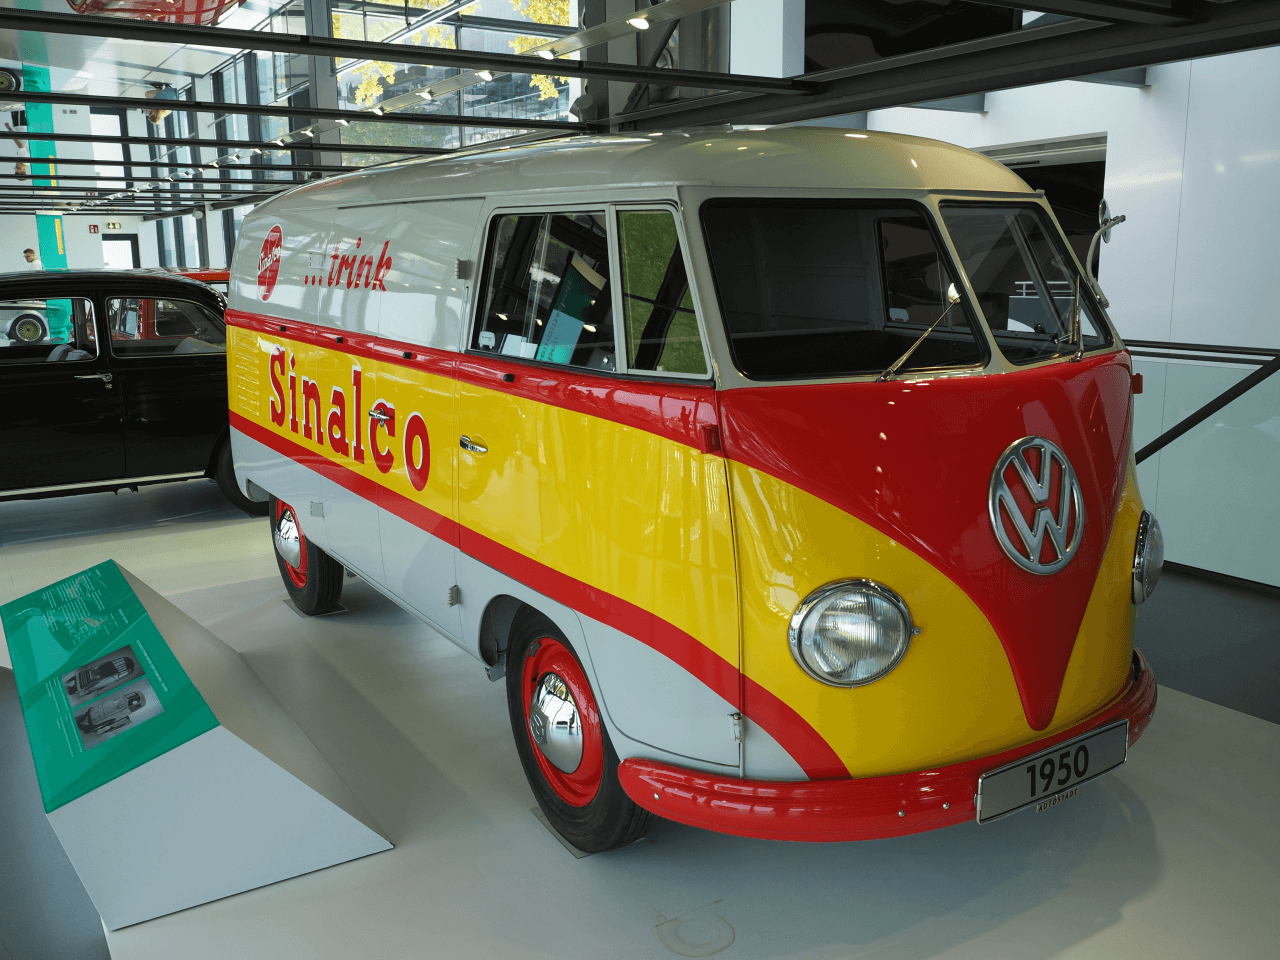
\includegraphics [width=0.3\textwidth]{../Bilder/Sylt/53.png}}\quad
   \subfloat{\includegraphics [width=0.3\textwidth]{../Bilder/Sylt/54.png}}\quad
   \subfloat{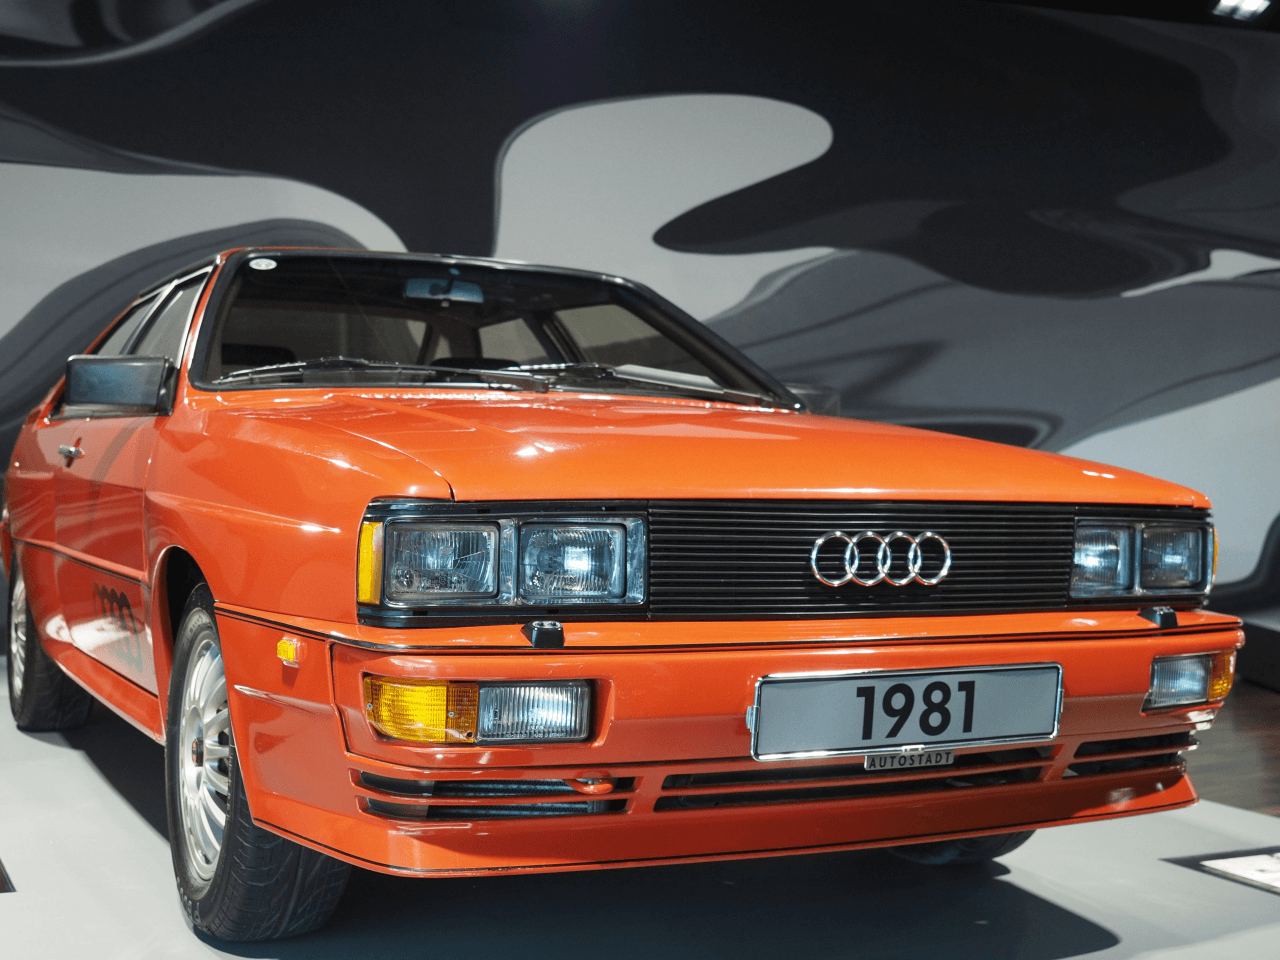
\includegraphics [width=0.3\textwidth]{../Bilder/Sylt/55.png}}\quad
   \caption[ZeitHaus]{ZeitHaus}
\end{figure}

In diesem Gebäude findet man ein Querschnitt der Automobil Geschichte.
Überhaupt nicht auf den Konzern aus Wolfsburg beschränkt.
Auf dem Gelände befindet sich zusätzlich ein Haus für die Marken Audi, Porsche, VW, VW Nutzfahrzeuge, Skoda, Seat, Lamborghini.
Die einzelnen Gebäude widerspiegeln immer die Marke selbst. 
Zusätzlich sind zwei Autotürme zu sehen in welchen die Fahrzeuge gelagert werden.
Kunden können in der Autostadt ihr Fahrzeug abholen und auch gleich auf einer internen Teststrecke kennenlernen.
Nach etlichen Stunden und noch mehr Fotos ging es zurück zum Bus um ein bisschen schlauer aus dem Buch \glqq You are not a gadget\grqq{} zu werden.
Das Nachtessen wurde direkt auf dem Campingplatz eingenommen, genauer neben dem Bus.
Spaghetti, zozusagen der Klassiker unter dem Camping Essen.
Danach wurde dieser Bericht geschrieben, das Geschirr abgewaschen und weiter im Buch gelesen.

\begin{figure}[H]
   \centering
      %\subfloat[CAPTION]{BILDERCODE}\qquad
   \subfloat{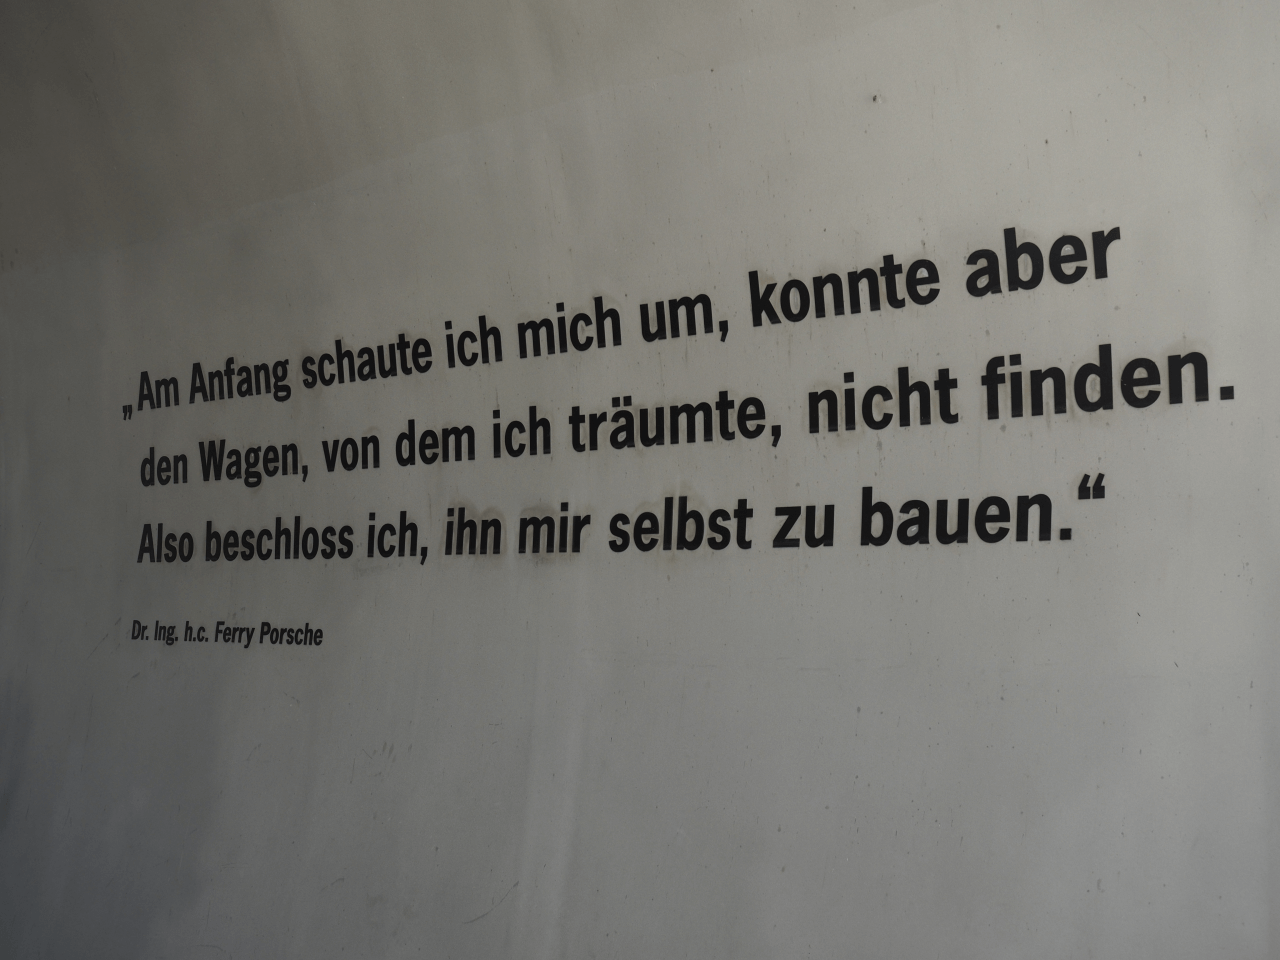
\includegraphics [width=0.3\textwidth]{../Bilder/Sylt/61.png}}\quad
   \subfloat{\includegraphics [width=0.3\textwidth]{../Bilder/Sylt/60.png}}\quad
   \subfloat{\includegraphics [width=0.3\textwidth]{../Bilder/Sylt/62.png}}\quad
   \caption[AutoStadt]{AutoStadt}
\end{figure}

\subsection{20.08.2018 Bomardement in Nürnberg}
Das mit dem frühen Aufstehen um loszufahren üben wir ein anderes Mal.
Kurz vor 9 Uhr gingen die Türen auf und nach einem kurzen Frühstück und einer noch kürzeren Dusche (nur kaltes Wasser) wurde alles wieder in den Bus gestopft und alles Fahrbereit gemacht.
Zuerst musste jedoch wieder einmal Jack mit Benzin versorgt werden.
Bei dieser Gelegenheit begab ich mich noch einmal (eher unfreiwillig) auf die Suche nach dem Stadtzentrum.
Bei einer Tankstelle angekommen wurde der Tank dann randvoll, oder doch eher über den Rand gefüllt.
Die Spritpumpe sprudelte ganz einfach zu lange.
Ein Schwall schoss aus dem Tankstutzen zurück und es tropfte dank der kaputten Entlüftung aus allen Poren des Busses.
In diesem Moment kommt ein zweiter T3 angefahren.
Die Frau steuert direkt auf mich zu und fragt ob ich bei ihrem Bus den Ölstand messen könne.
Der Bus hätte auf einmal komisch geklungen auf der Bahn.
Er sei auch nur gemietet.
Ich konnte die gute Frau vorerst beruhigen.
Der Ölstab erreichte das Öl problemlos und sie konnte ihre Reise fortsetzen.
Unter meinem Bus hatte sich der weilen ein kleiner See gebildet.
Schnell bezahlt und ab die Post damit der Sprit verbrannt und nicht flüssig in die Umwelt entlassen wird.
Kilometer reihte sich an Kilometer, glücklicherweise ohne Stau.
Nach einem Halt in einer Autobahnraststätte in der sich eine eher älter Dame über die Geschwindigkeit der Kassiererin beschwerte, welche gelassen konterte: Dann bewerben sie sich doch hier, erreichte ich Nürnberg bei strahlendem Sonnenschein.
Der grössere Campingplatz ist auf dem 11km$²$ ehemaligen Reichsparteitaggelände gelegen.
Nach dem Aufstellen wollte ich sofort Nürnberg besichtigen, was ich nach einem Nickerchen auch tat.
Mit dem Fahrrad ginge es zuerst durch  den Wald am Stadion vorbei auf die grosse Strasse.
Eine Strasse welche den Namen auch verdient: 60m breit und 2 km lang mit Granitplatten ausgelegt.

\begin{figure}[h]
    \centering
    \includegraphics[width=0.7\textwidth]{../Bilder/Sylt/71.png}
    \caption{Grosse Strasse}
    \label{img:Grosse Strasse}
\end{figure}

\newpage

Danach stand ich vor der Kongresshallle in der heute das Museum \glqq Dokumentationszentrum\grqq{} untergebracht ist. 
Nach einer Fahrt von 15min kam ich in der Altstadt an und stürchelte sofort über einen Pizzastand.
Ein paar Fotos später ging es auch schon zurück zum Campingplatz.

\begin{figure}[h]
    \centering
    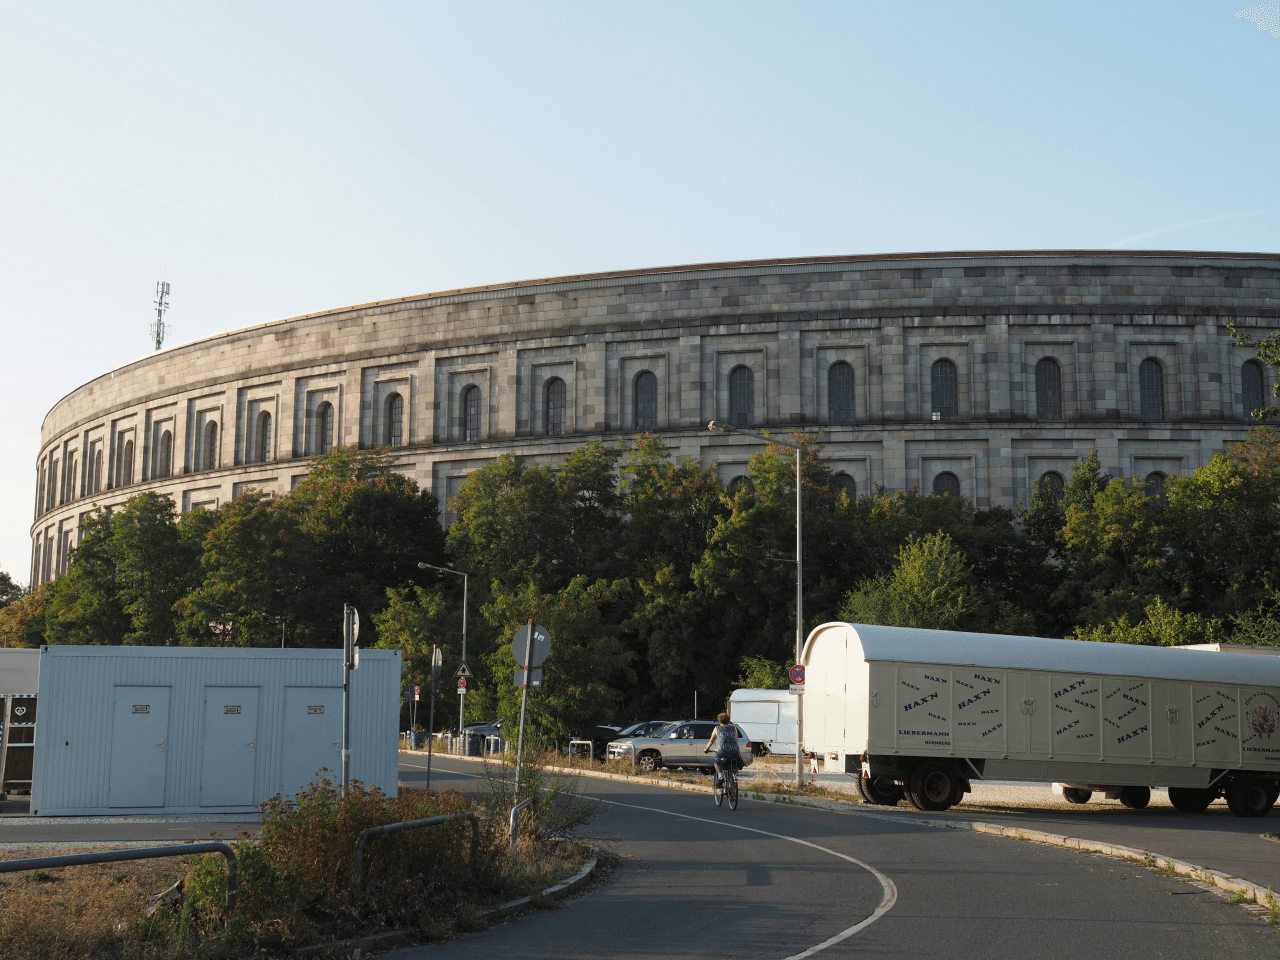
\includegraphics[width=\textwidth]{../Bilder/Sylt/65.png}
    \caption{Konresshaus}
    \label{img:Konresshaus}
\end{figure}

Nach dem Besuch der Stadt Nürnberg genoss ich vor dem Bus noch ein paar Minuten die kühle Brise
Die kühle Brise sollte sich aber schon bald als hinterhältig herausstellen.
Der ganze Campingplatz ist umsäumt von Eichen.
Diese Schattenspender besitzen eine lustige Frucht, welche durch den Wind gelöst mit Getöse auf den Boden knallt.Solange nur der Boden getroffen wird ist alles in Ordnung,
Mit Regelmässigkeit wird jedoch ein Fahrzeug getroffen.
Schön erkennbar an einem lauten Knall.
So sass ich nun vor dem Bus und um mich herum herrschte Krieg
Ein kurzes Knacken in den Bäumen und dann irgendwo der Einschlag.
Hier sollte ein Schild aufgestellt werden: Helmpflicht.
Der Wind nahm zu und ich musste mich in Sicherheit vor dem Bombardement bringen.

\newpage 

\subsection{21.08.2018 Größenwahnsinn nahe erlebt}
Nach einer kalten, klaren Nacht und einem Frühstück an der Sonne wollte ich das Dokumentationszentrum anschauen.

\begin{figure}[H]
   \centering
      %\subfloat[CAPTION]{BILDERCODE}\qquad
   \subfloat{\includegraphics [width=0.45\textwidth]{../Bilder/Sylt/66.png}}\quad
   \subfloat{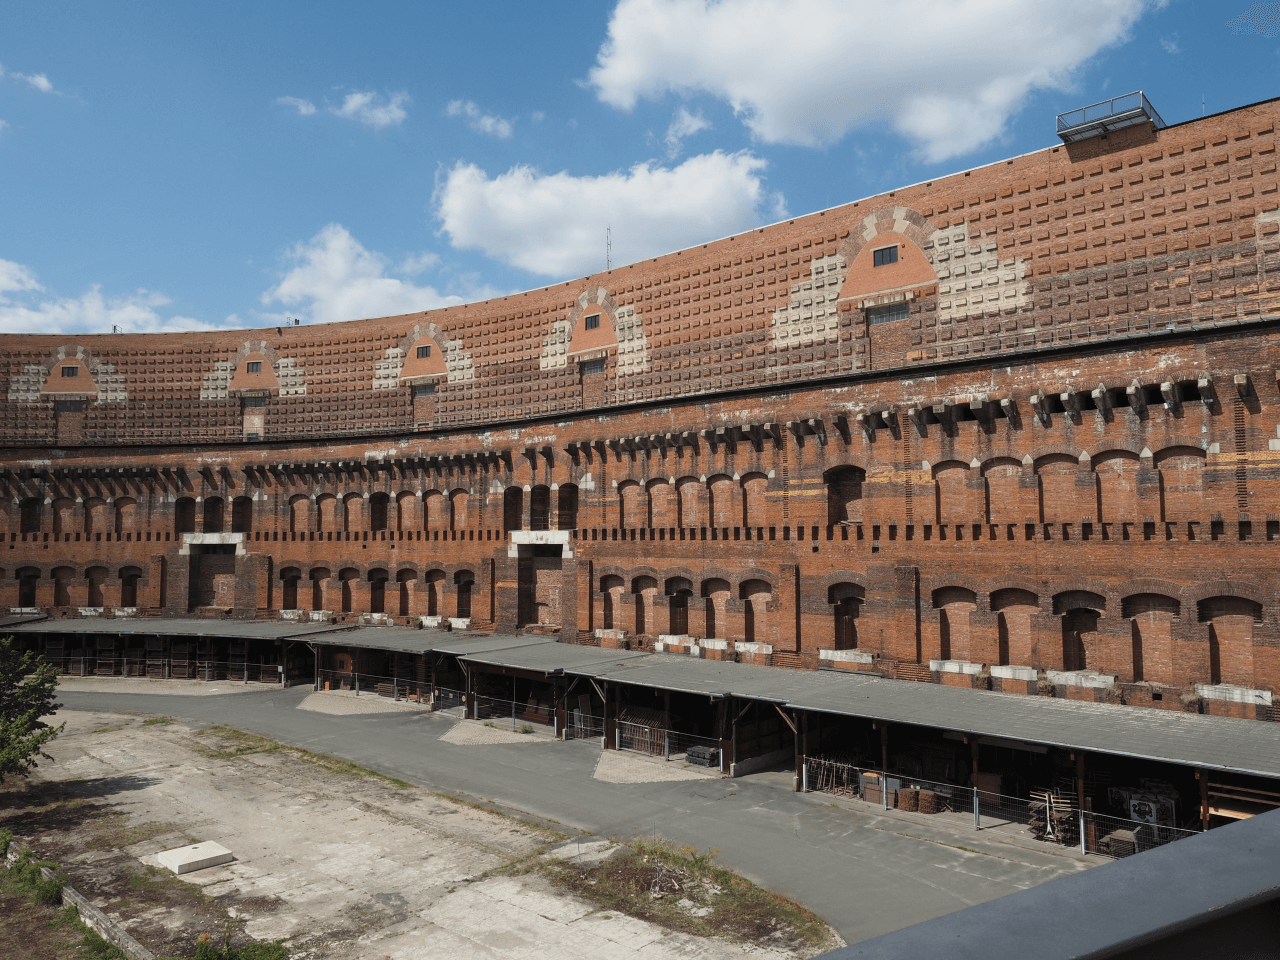
\includegraphics [width=0.45\textwidth]{../Bilder/Sylt/67.png}}\quad
   \caption[Dokumentationszentrum]{Dokumentationszentrum}
\end{figure}

Die Strecke war ja wohlbekannt und schon bald stand ich in dem riesigen nie fertiggestellten Gebäude.
3h und jede Menge Informationen später kam ich beim Ausgang des Museums an.
Geschichte verbunden mit den Gebäude und den gezeigten Filme und Fotos ist sehr eindrücklich und erschreckend.
Schön ist da jetzt unter anderem wieder ein Campingplatz drauf und keine 100'000 Soldaten.
Das Bistro versorgte mich mit dem Nötigsten.
In diesem Fall mit einer wunderbaren Gulaschsuppe.
Den bekannten Weg in die Altstadt kannte ich schon und so versuchte ich mich an einer Alternative.
Erfolgreich kam ich so am Fusse des Hügels an, auf dem die Burg steht.
Per pedes wurde auch diese erkundet und danach die Altstadt und die Einkaufsmeile.
Den Rucksack ein weiteres Mal mit allerlei Getränken vollgestopft und gestärkt durch eine Currywurst trat ich bei bestem Wetter den Rückweg an.
Am Abend nach der Dusche und einem feinen Nachtessen im Campingrestaurant bereitete ich schon die ersten Dinge für eine möglichst frühe Abfahrt am Mittwoch vor.

\begin{figure}[H]
   \centering
      %\subfloat[CAPTION]{BILDERCODE}\qquad
   \subfloat{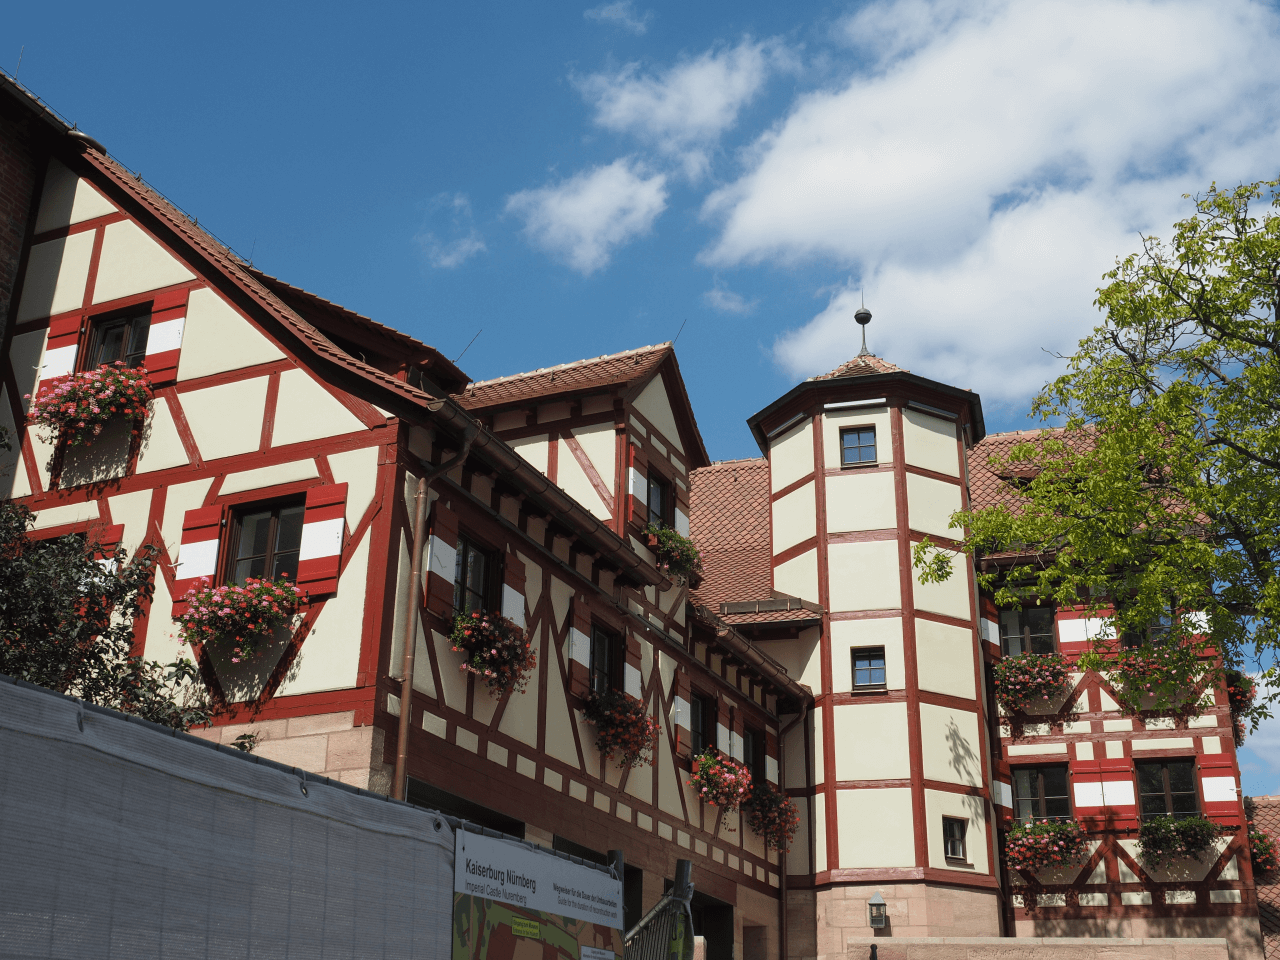
\includegraphics [width=0.45\textwidth]{../Bilder/Sylt/69.png}}\quad
   \subfloat{\includegraphics [width=0.45\textwidth]{../Bilder/Sylt/70.png}}\quad
   \caption[Altstadt]{Altstadt}
\end{figure}

\newpage

\subsection{22.08.2018 Fahrt nach Hause}
Schon um halb Sieben klingelte der Wecker.
Auch dieses Mal klingelte er erfolglos.
Trotzdem war ich kurz vor Acht schon unterwegs.
Mit dem Bus die grosse Strasse zu befahren, eher ungewöhnlich und holprig.
Die weitere Fahrt zog sich zwar in die Länge war sonst aber absolut problemlos.
Fast ein wenig zu problemlos \dots
Um den Hunger zu stillen wurde kurzerhand ca. 900m vor der Haustüre ein Kebabstand angepeilt und mit dem Bus direkt davor parkiert.
Die Augen nur auf das Essen gerichtet stürmte ich den kleinen Laden.
Vor der Türe wurde ich von einer älteren netten Dame darauf aufmerksam gemacht, dass das Licht noch an sei.
Ich erwiderte freundlich, dass das schon in Ordnung ist.
Nach dem Bezahlen zurück in den Bus gehüpft, Schlüssel gedreht und überhaupt nichts passierte.
Verd \dots
Was sollte dass jetzt so kurz vor dem Ende der Reise?
Einen Blick auf die Spannungsanzeige der Startebatterie riskiert: 12,7V
Alles tip top.
Die ältere Dame schaut schon schräg zu mir rüber.
Muss ich jetzt wirklich da Fragen gehen ob sie mir beim Anschieben helfen würden?
Doch eher peinlich.
Was könnte denn das Problem sein?
Ok ein paar Minuten warten hat noch nie geschadet.
Half alles nichts.
Naja, schauen wir einmal die Batterie an.
Was sahen meine müden Augen da:
Zerschmolzenes, stinkendes Plastik.
Der Sicherungshalter für die Zuleitung des Batterieladegerät hatte sich verflüssigt.
Wieso sollte der Bus denn so nicht starten?
Egal die Leitung mit dem Seitenschneider gekappt.
Rums lief die Büchse wieder und die letzten Meter konnten noch zurückgelegt werden.

Nach dem Ausräumen musste dafür einen Ersatz für den Sicherungshalter und das kaputte Kabel gefunden werden.

\subsection{Fazit}
\begin{itemize}
     \item Auch 2500km Fahrt können einem alten VW Bus nichts anhaben
     \item Ab 120 km/h wird man auf deutschen Autobahnen komisch angeschaut wenn man einen T3 fährt
     \item Was Jesus konnte, können wir schon lange --> Wanderung von einer Insel zu anderen
     \item Es gibt schöne und weniger schöne Städte in Deutschland
     \item Leuchttürme blenden ungemein in der Nacht
     \item Eichen spenden zwar Schatten, verursachen dafür Dellen im Blech
     \item Mann soll die Ausfahrt nicht 900m vor dem Ende als problemlos abstempeln
     \item Bus läuft und läuft und läuft, mein Gebastel geht doch öfters kaputt.
\end{itemize} 
